
\section{Results}

\subsection{Image}

\subsubsection{Growth of images in Docker hub}

Figure~\ref{fig_image_growth} show the total number of images in Docker hub increases from May 30th to Sept. 20th 2017. As discussed in~\cite{XXX}, Crawler searched for `/' by using Docker hub search engine, crawled the web page, and obtained the total number of non-official public repositories in Docker hub each day. By summing both official repository count and non-official repository count, we got the total number of repositories in Docker hub each day. As shown, the total number of repositories increased from 633,915 on May 30th to 687,292 on Jul. 11th with ~1,241 repositories created per day.

\begin{figure}
  \centering
  % Requires \usepackage{graphicx}
  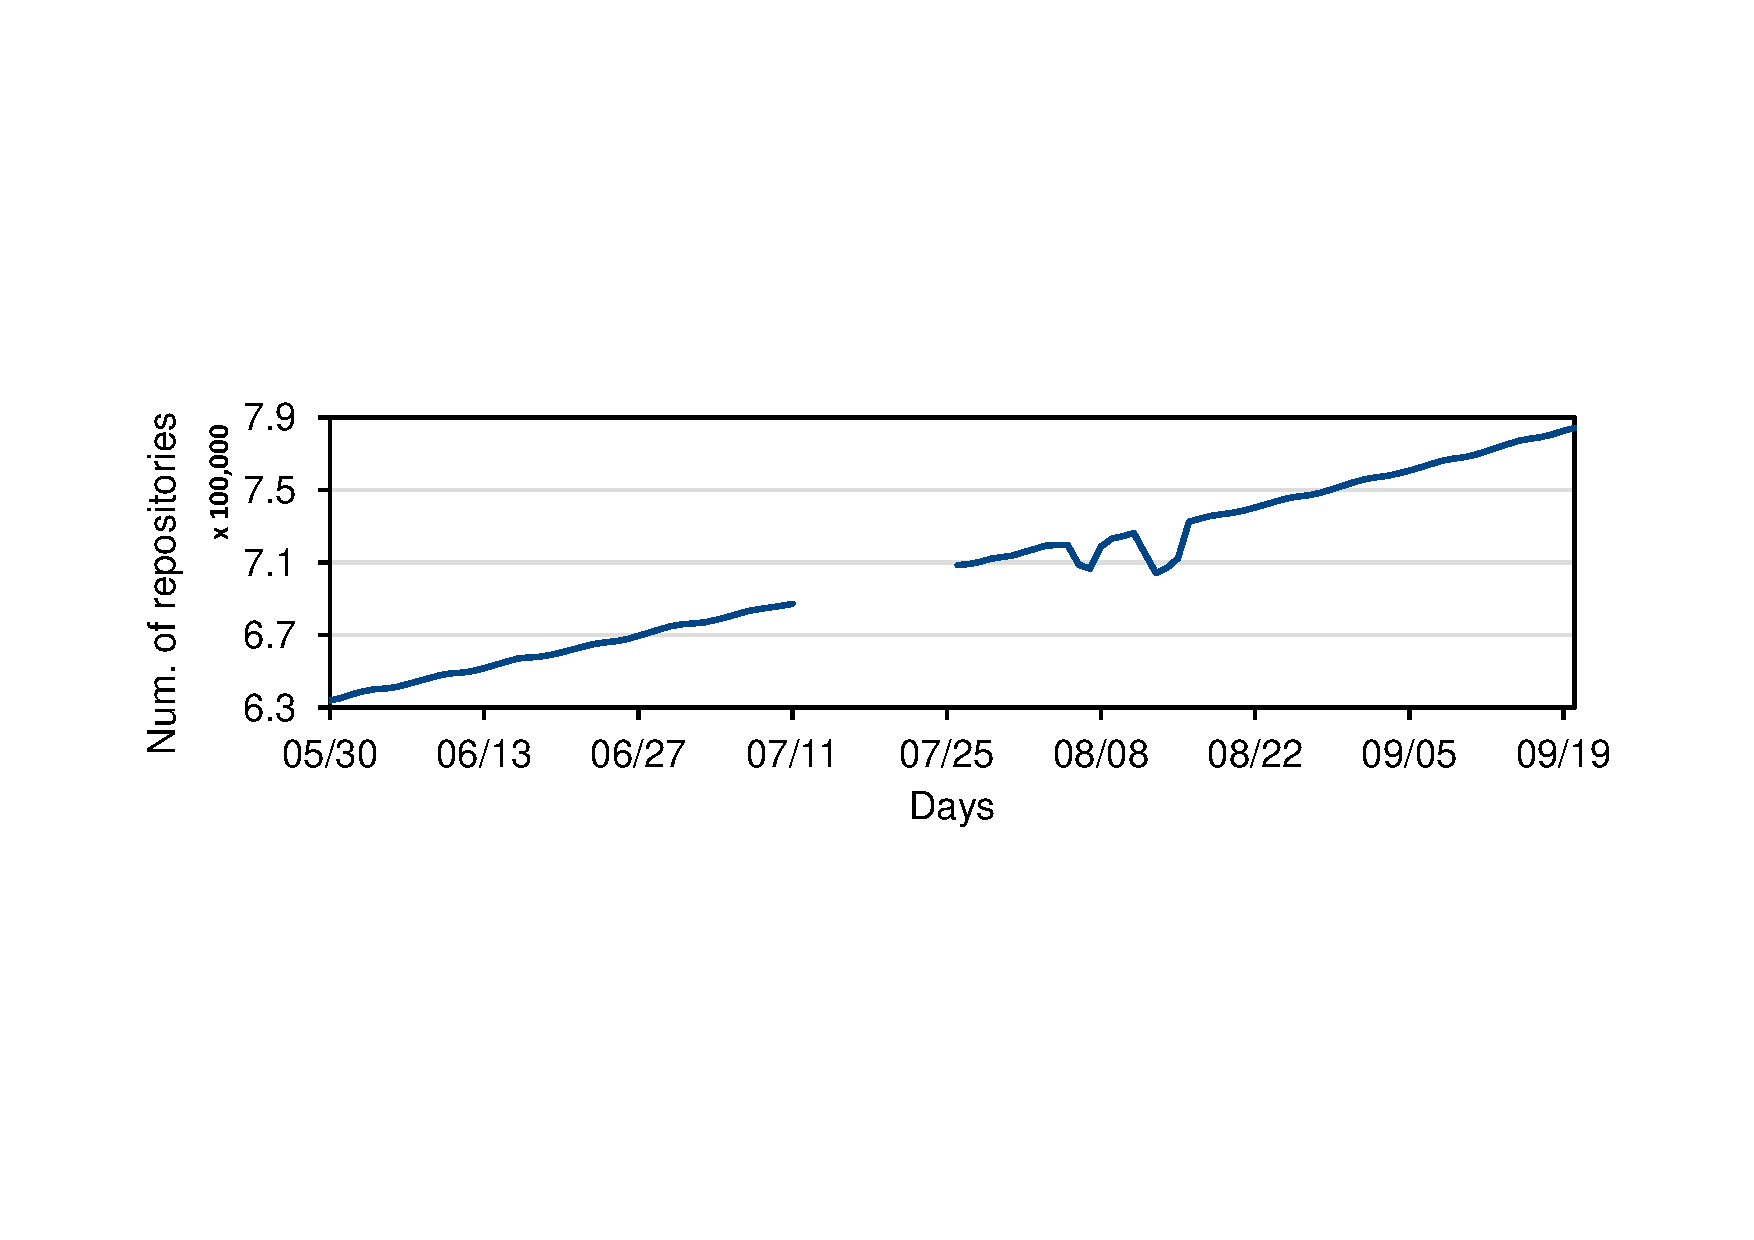
\includegraphics[width=0.5\textwidth]{graphs/image_growth.pdf}
  \caption{Total number of repositories in Docker hub from May 30th to Sept. 20th}\label{fig_image_growth}
\end{figure}

A interesting observation is that Crawler can get a similar list of images if we replace `/' with `*'. Note that from 5/30/2017-7/11/2017, Crawler used above method to obtain the total amount of images in Docker Hub. But after 7/11/2017, the Docker Hub removed the index of `/'. Thus, currently we search for `*' instead of `/' to obtain a list of non-official public images. As shown in figure~\ref{fig_image_growth}, the total number of repositories increased from 708,647 on Jul. 26 to 784,182 on Sept. 20, with ~1,325 new repositories created per day. Overall, the total number of repositories is increasing, although there are two troughs during the period of 08/06-08/07 and 08/13-08/15.

\subsubsection{Image popularity distribution}

Figure~\ref{fig-pop} shows the repository popularity distribution by May 31th. The x-axies show the pull count (i.e., total number of pulls) for repositories by May 31th with different ranges.
Figure~\ref{fig_pull_cnt_total} shows the cumulative repository frequency by pull count. ~95\% of the repositories are pulled than 1000 totally. 90\% of the repositories only have a pull count less than 333. The greatest pull count is 654,088,410, which is official repository~\textit{nginx}. 
Figure~\ref{fig_pull_cnt_count} shows the repository frequency by pull count. 31,200 of repositories are not at all.  
34,100 repositories are pulled only ~4 times and 27,600 repositories are pulled ~37 times, which are the two peaks shown in the figure.
Overall, repository frequency decreases with the pull count.

The skewness of two curves in figure~\ref{fig-pop} suggests that Docker hub is a good fit for caching few popular repositories or images, which can significantly improve the \textit{pull} or \textit{push} performance.      

\begin{figure}[!t]
	\centering
	\subfigure[CDF of repositories by pull count]{\label{fig_pull_cnt_total}
		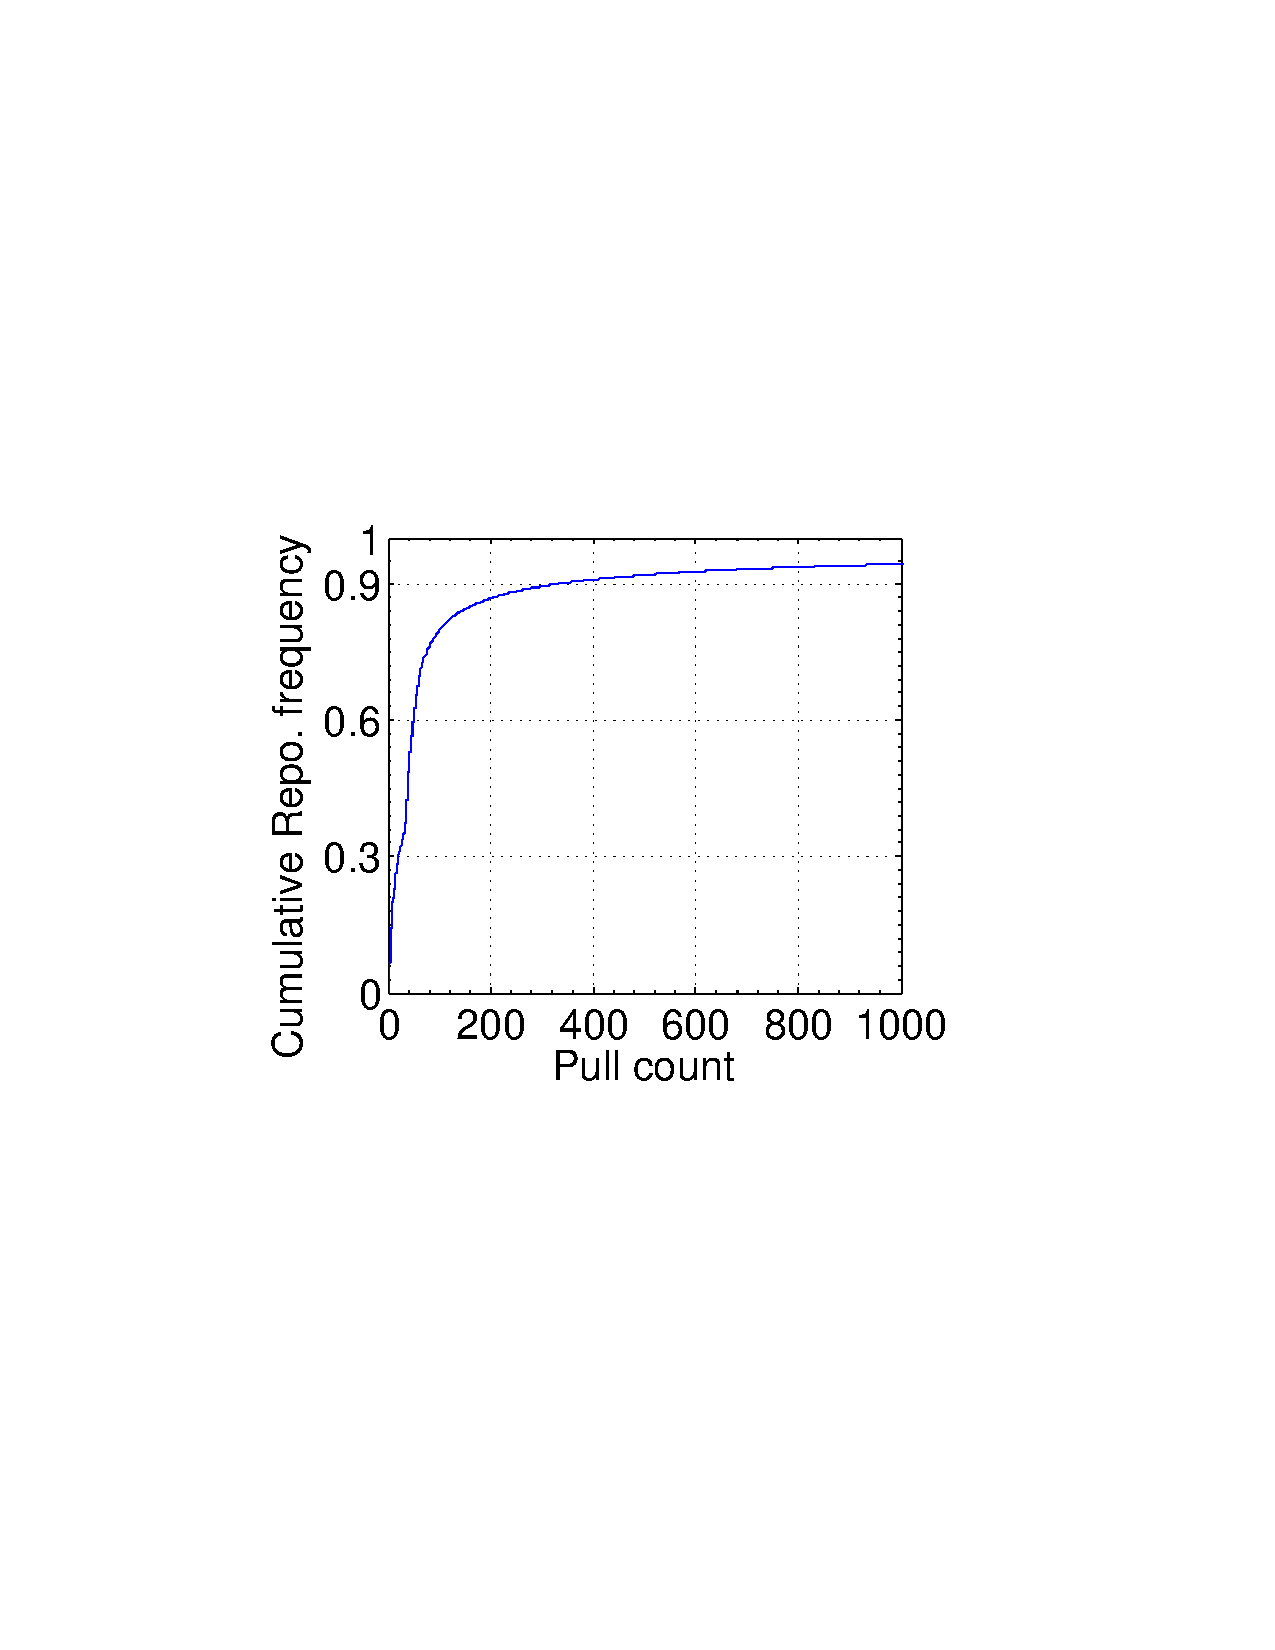
\includegraphics[width=0.23\textwidth]{graphs/pull_cnt.pdf}
	}
	\subfigure[Histogram of repositories by pull count]{\label{fig_pull_cnt_count}
		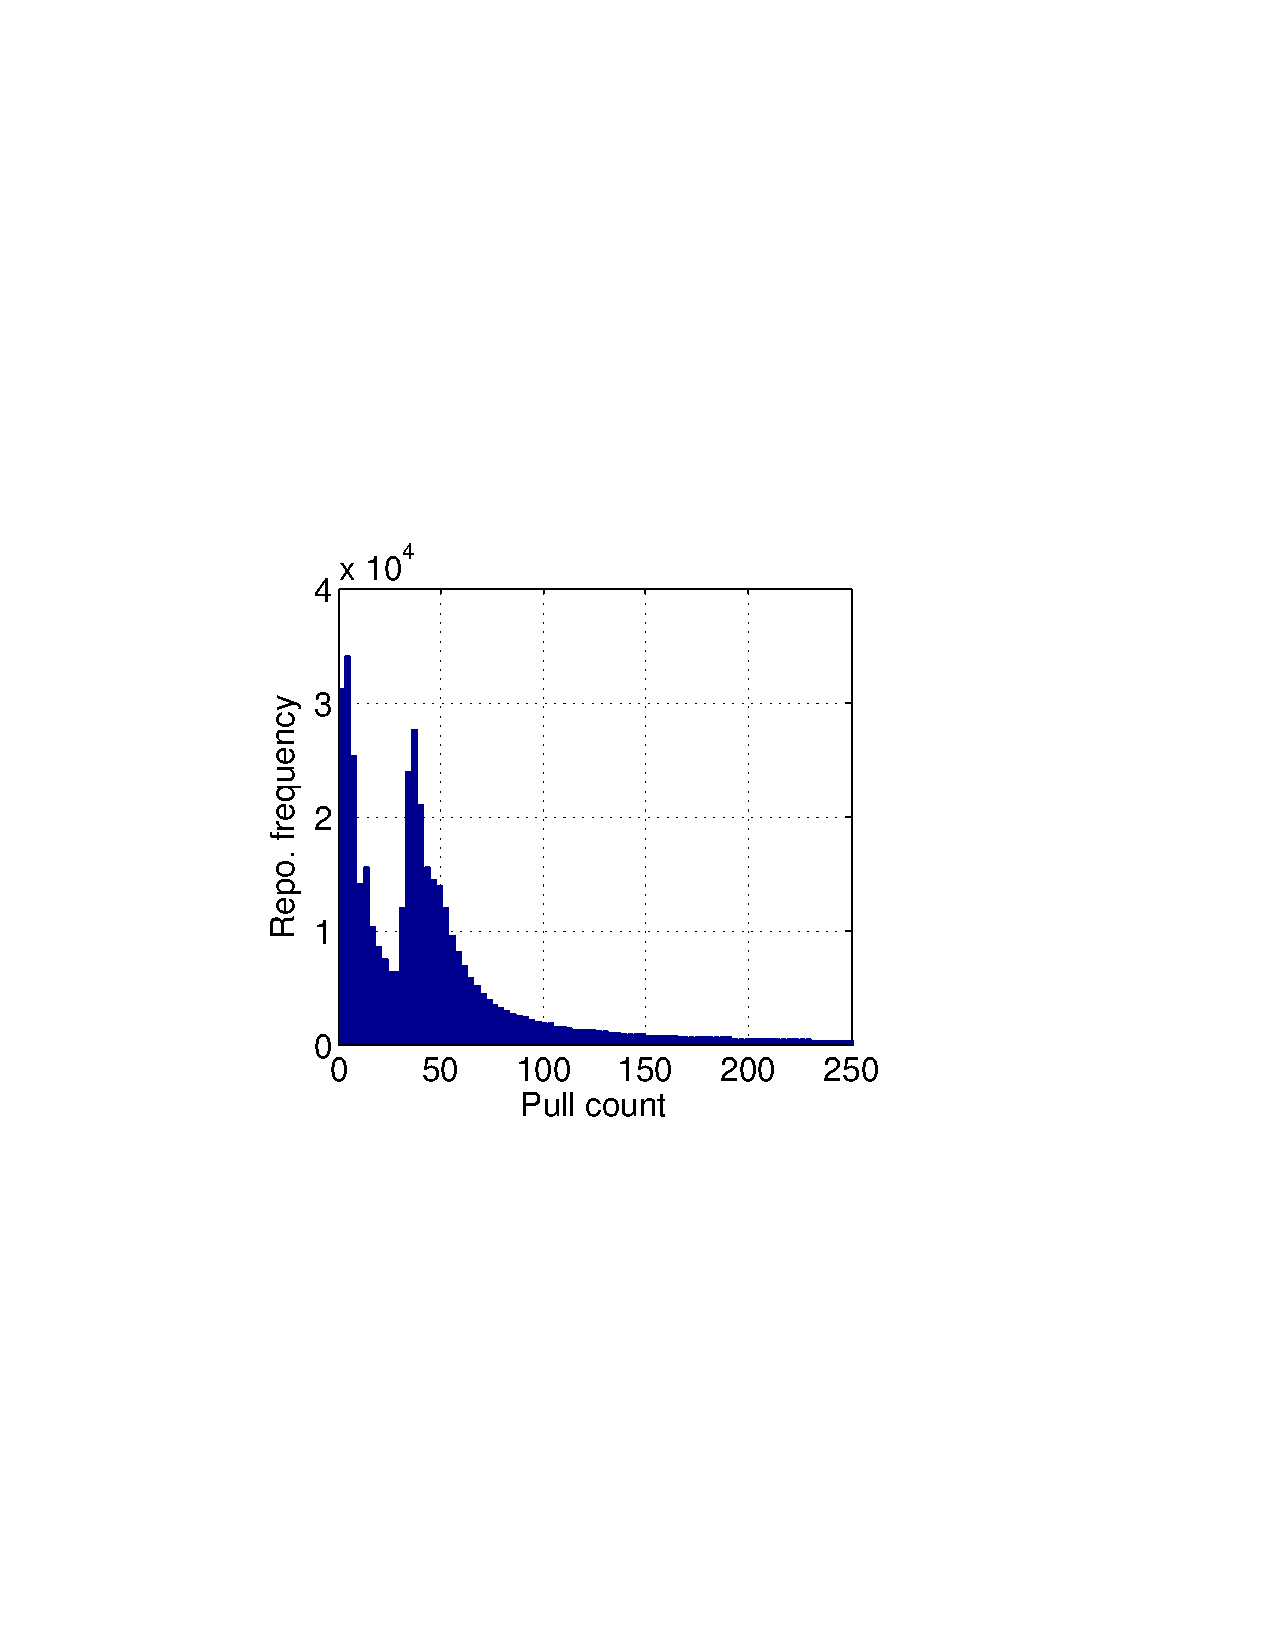
\includegraphics[width=0.22\textwidth]{graphs/count_pull_cnt.pdf}
	}
	\caption{Repository popularity distribution}
	\label{fig-pop}
\end{figure}

\subsubsection{Image size distribution}
\label{sec:image-size}
We measured three kinds of image size: archival size, compression size, and the sum of containing file size. Compression size is the sum of its containing \textit{gzip} compressed layer size (i.e., original layer size after downloaded); The archival size is the sum of its containing decompressed layer size (i.e., decompressed layer size without extracting and unpacking); The sum of containing file size is the sum of its containing file size after decompression with extracting and unpacking.

Figure~\ref{fig-image-size} shows the cumulative image frequency by two scales (GB and MB) for three kinds of image size.
As shown in figure~\ref{fig_image_size_gb}, the red curve and blue curve are almost overlapped, which means that the distribution of archival size and the distribution of sum of file size are similar. 90\% of images have a less than 1.3GB uncompression size (i.e., archival size or the sum of containing file size), while 90\% of images have a less than 0.48 GB compression size. The largest uncompression image size is ~498 GB while the largest compression size is only 202 GB.
Figure~\ref{fig_image_size_mb} shows the cumulative image frequency by MBs. 70\% of the images have a less than 190 MB compression size. And 70\% of the images have a less than 478 MB uncompression size (i.e., archival size or the sum of containing file size). Half of the images have a less than ~17 MB compression size. Half of the images have a less than 46 MB archival size and 94 MB sum of containing file size.

Figure~\ref{fig-image-size} shows that the majority of the images in Docker hub have a smaller size. 90\% of images can be compressed with less than 500 MB and 70\% of images are less than 500 MB even without compression. 

\begin{figure}[!t]
	\centering
	\subfigure[CDF of images by size (GB)]{\label{fig_image_size_gb}
		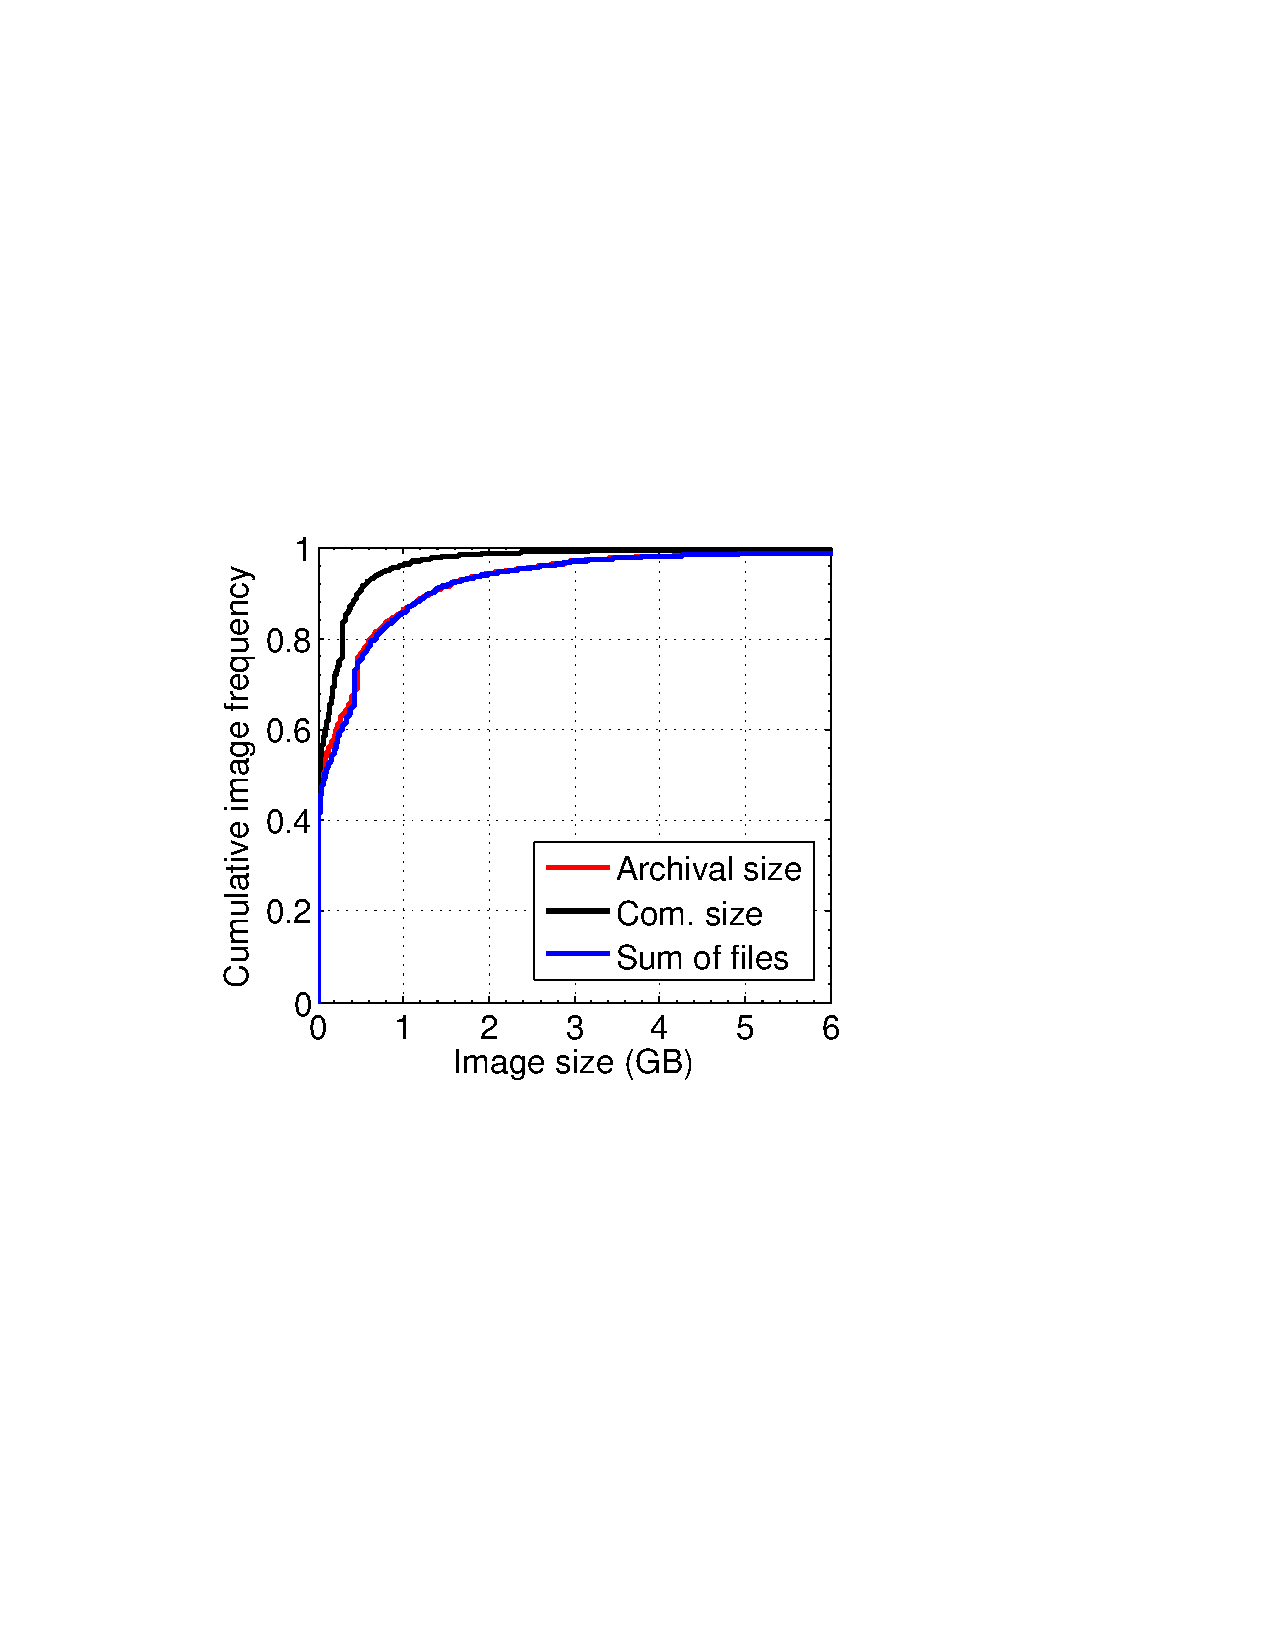
\includegraphics[width=0.22\textwidth]{graphs/image_size.pdf}
	}
	\subfigure[CDF of images by size (MB)]{\label{fig_image_size_mb}
		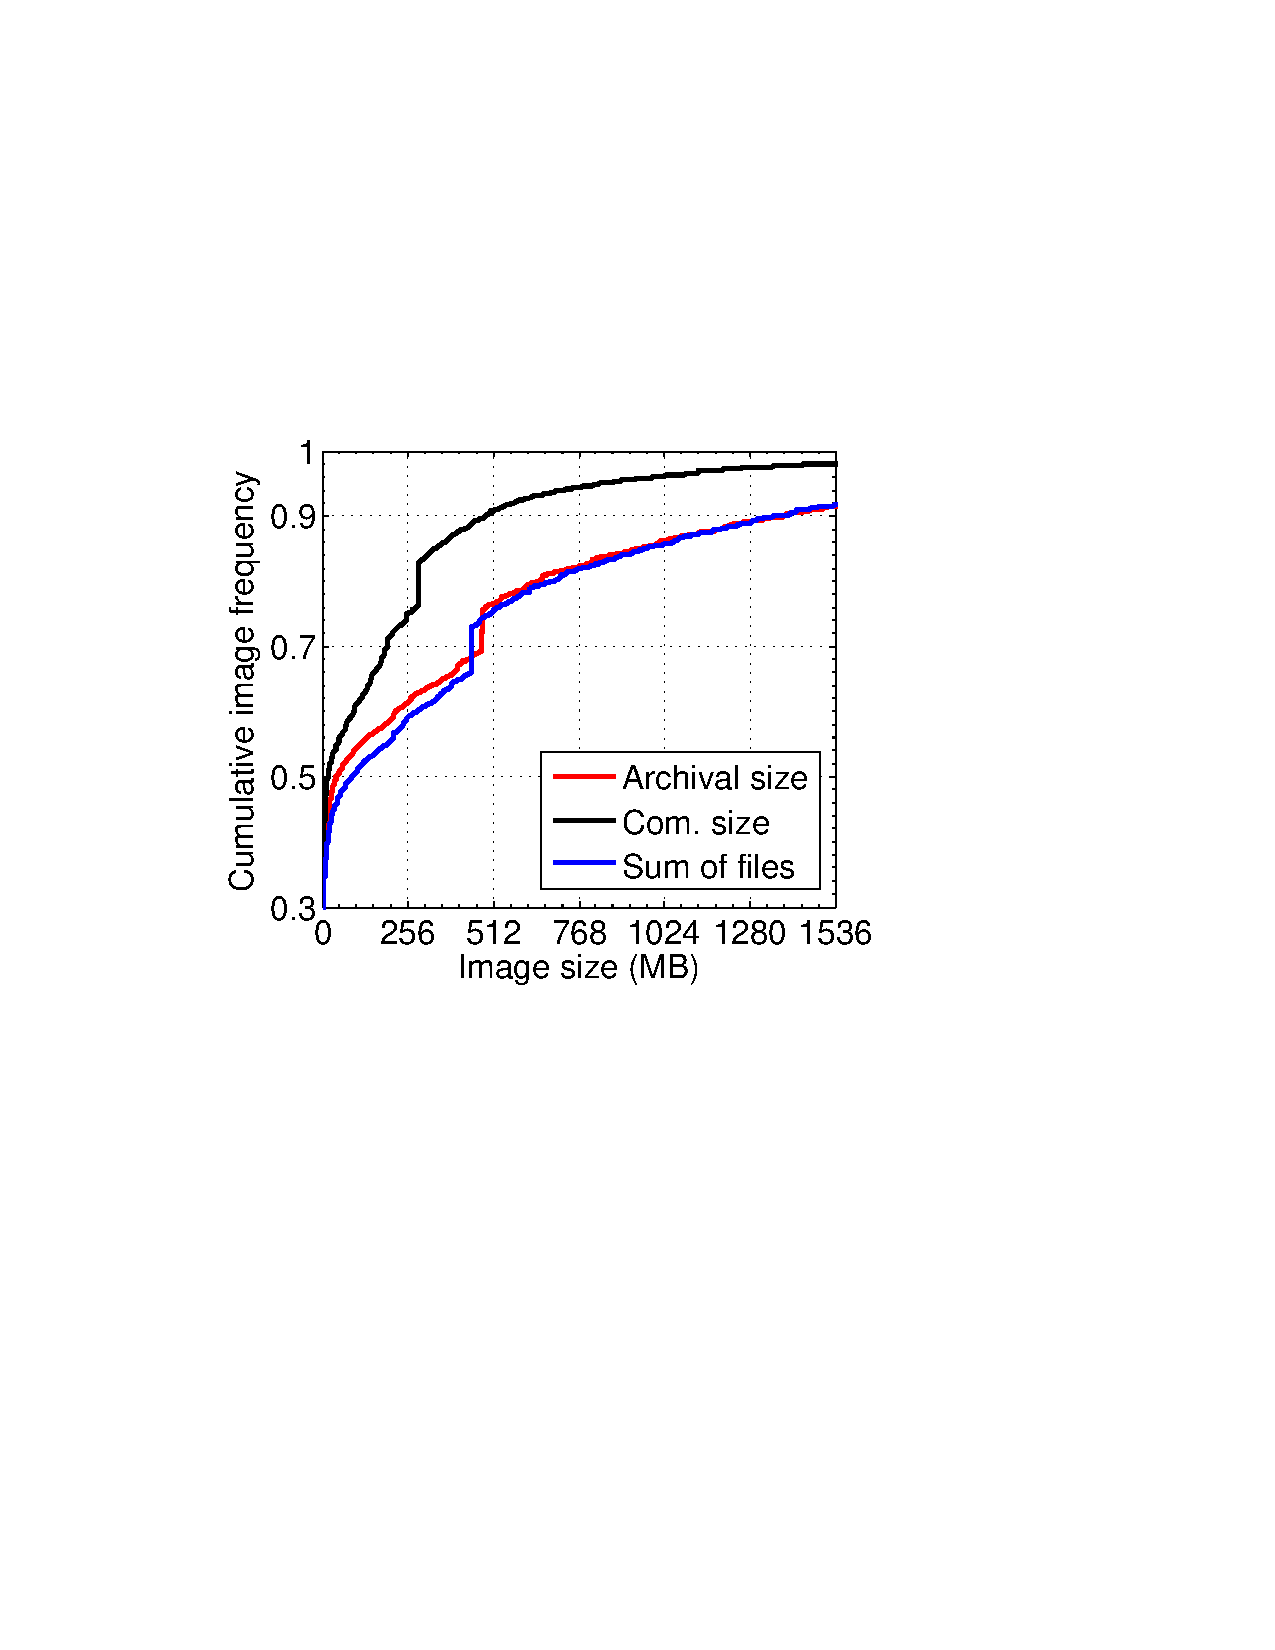
\includegraphics[width=0.23\textwidth]{graphs/image_size_mb.pdf}
	}
	\caption{Image size distribution}
	\label{fig-image-size}
\end{figure}

\subsubsection{Compression rate distribution}

\begin{figure}[!t]
	\centering
	\subfigure[CDF of images by compression ratio]{\label{fig_image_compression_ratio}
		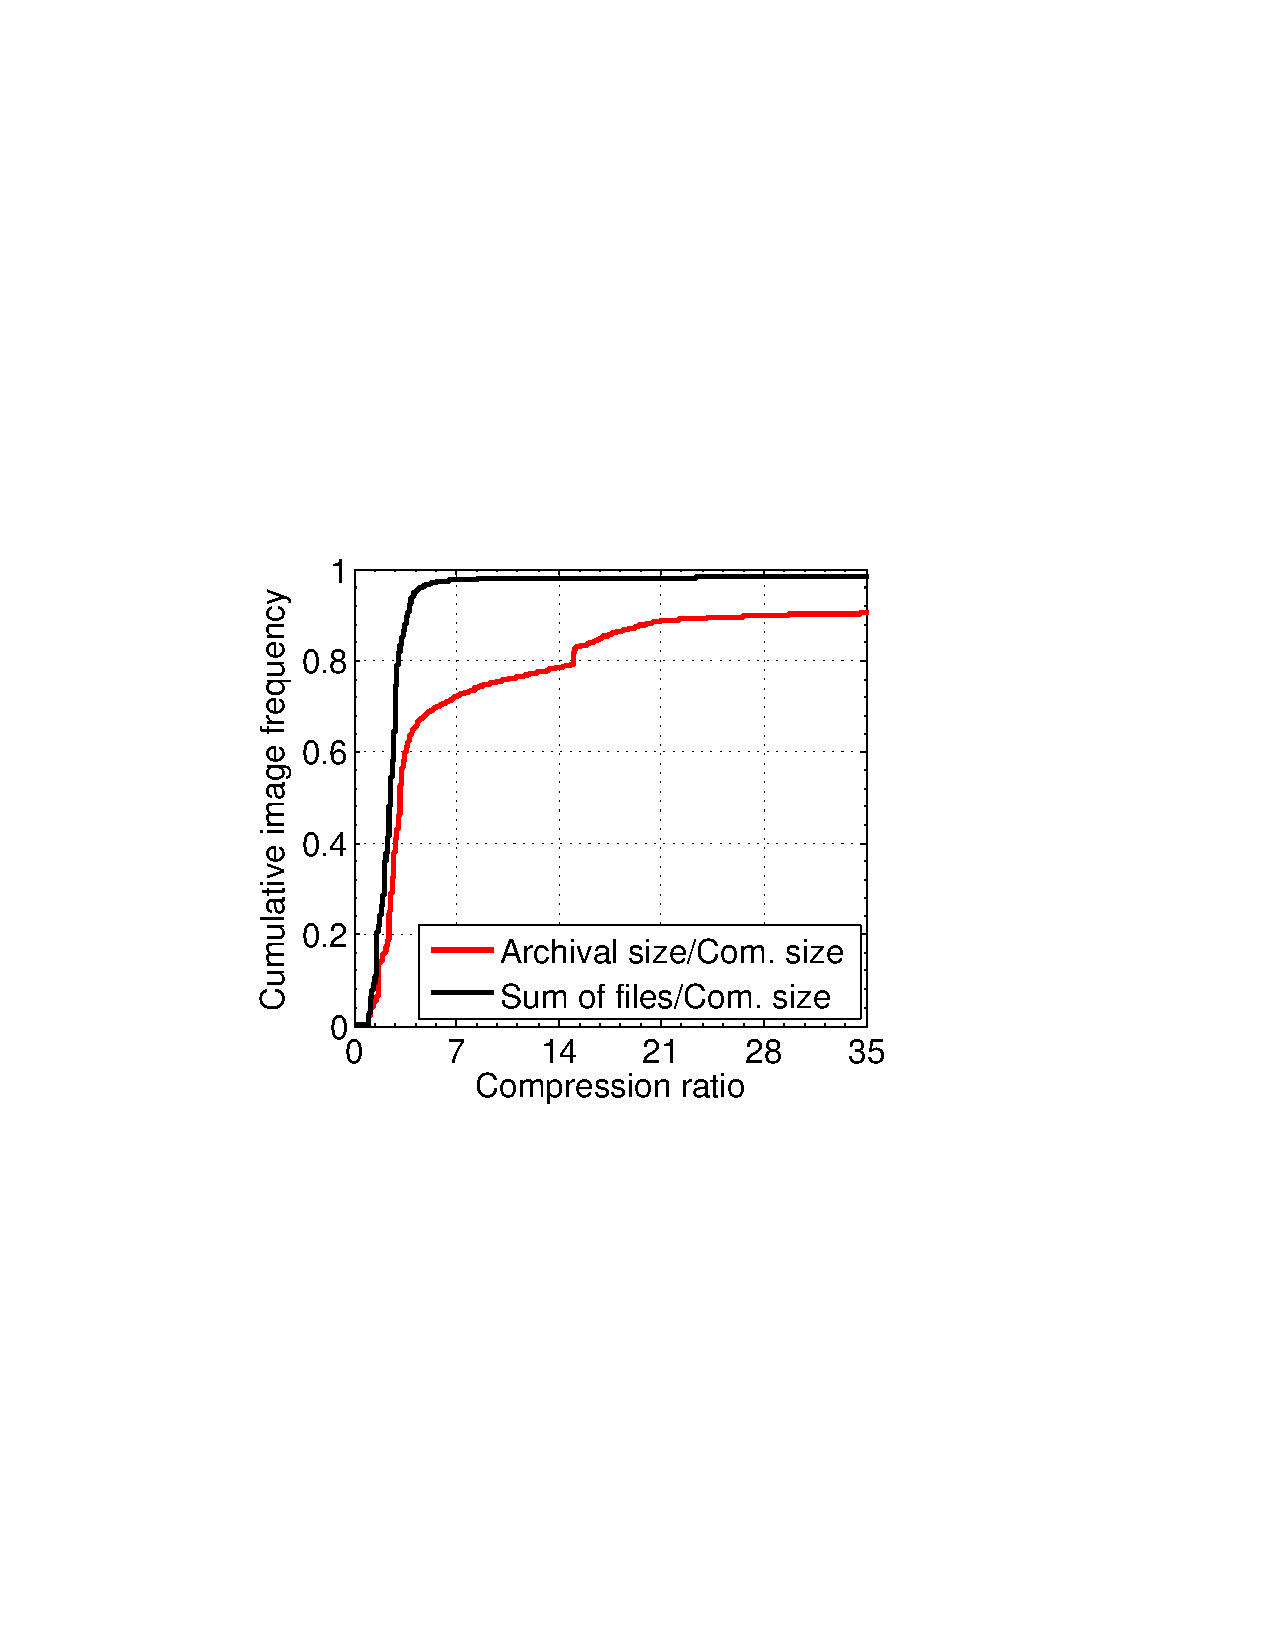
\includegraphics[width=0.23\textwidth]{graphs/image_compression_ratio_less.pdf}
	}
	\subfigure[Histogram of images by compression ratio]{\label{fig_image_compression_ratio_less}
		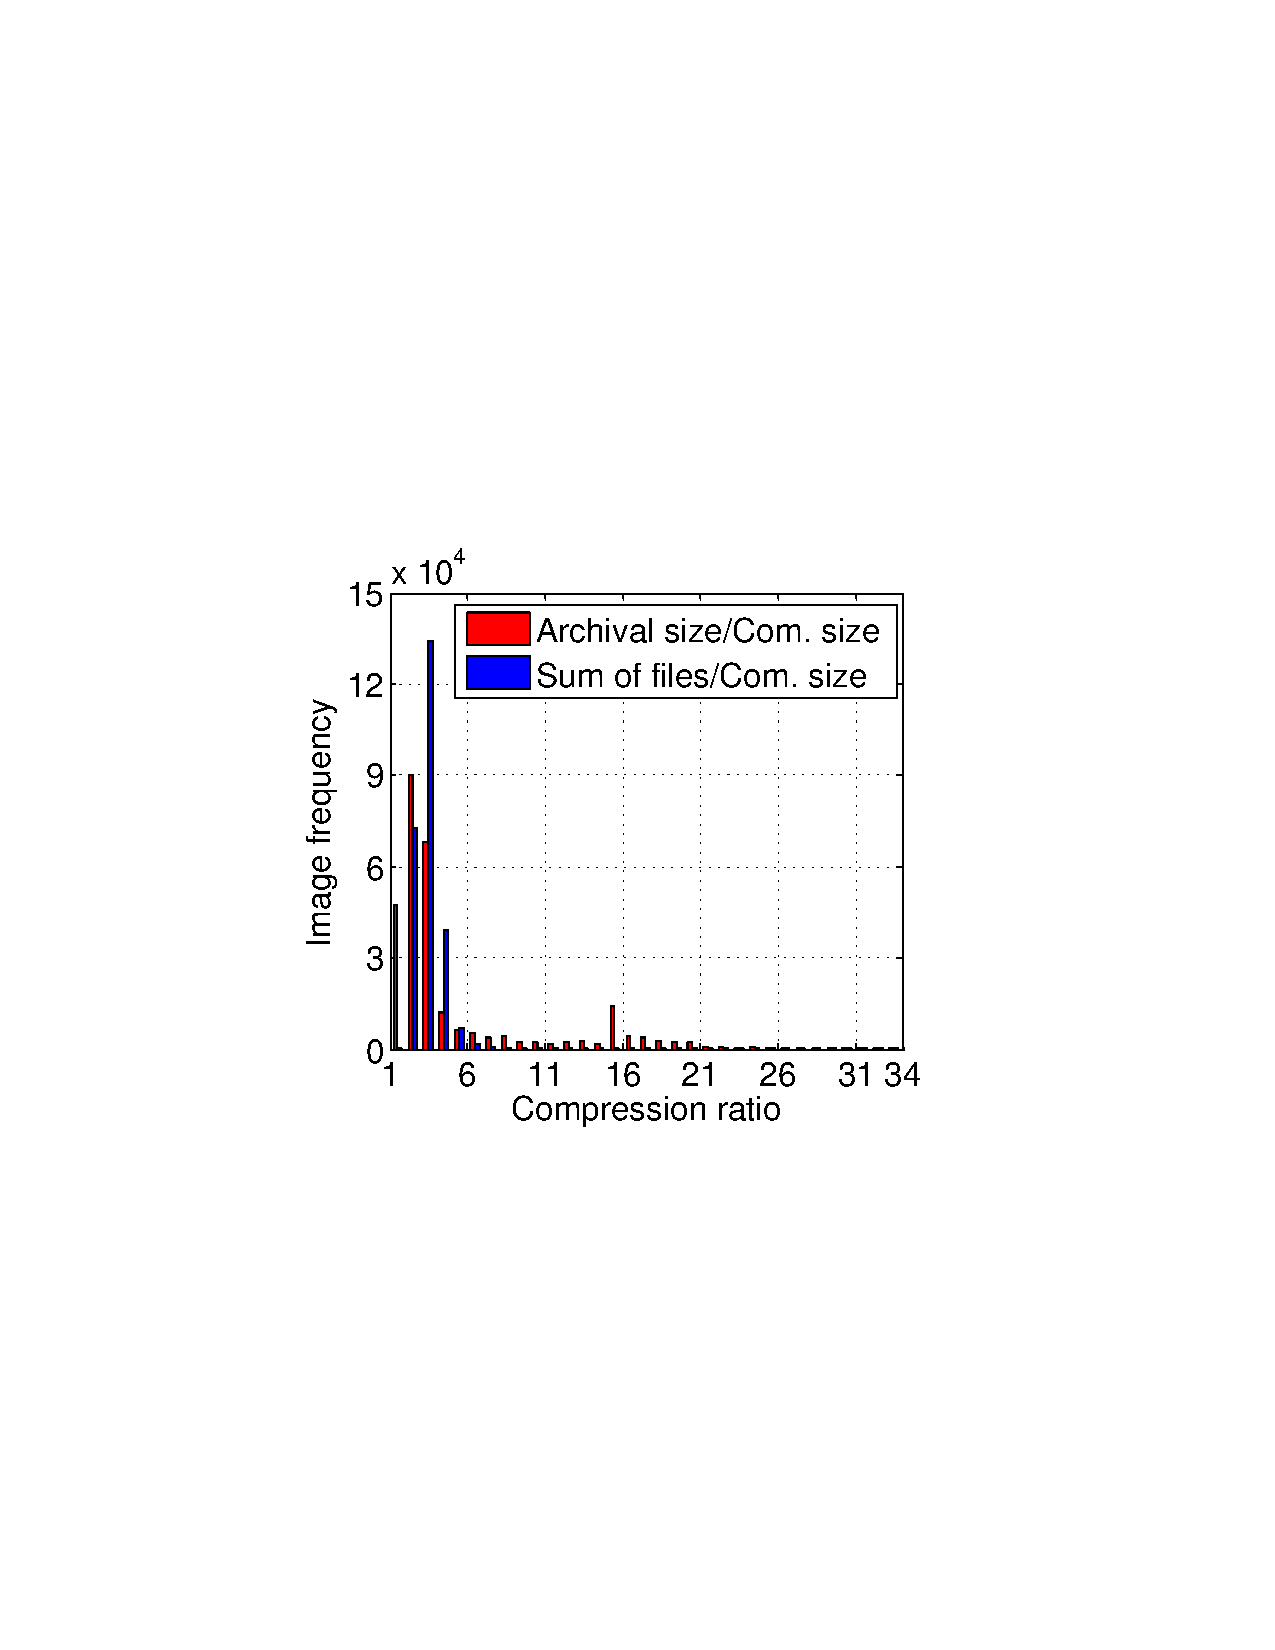
\includegraphics[width=0.223\textwidth]{graphs/hist_compression_ratio.pdf}
	}
	\caption{Compression rate distribution}
	\label{fig-image-compression-ratio}
\end{figure}

As discussed in~\ref{sec:image-size}, three kinds of image size are measured: archival size, compression size, and the sum of containing file size. Thus, we calculated two kinds of compression ratio: the ratio of archival size to compression size and the ratio of Sum of file size to compression size. 

Figure~\ref{fig-image-compression-ratio} shows the cumulative image frequency by compression ratio. Overall, we can see that the ratio of archival size to compression size is greater than the ratio of the sum of file size to the compression size. 90\% of images have a archival-to-compression ratio less than ~4 while 90\% of images have a sum of file-to-compression ratio less than 35. Half of the images have a compression ratio (both archival-to-compression and sum of files-to-compression) around 3. The maximum compression ratio are 512,930 and 1028 for the ratio of sum to file size to compression size and the ratio of archival to compression size respectively.
Figure~\ref{fig_image_compression_ratio_less} shows a histogram of image frequency by compression ratio. 134,000 images have a ratio of sum of file size to compression size of 3.5 and 90,000 images have a ratio of sum of archival size to compression size of 2.5, which are two peaks shown in the graph.

Figure~\ref{fig-image-compression-ratio} suggests that Docker images has a great potential for compression to save space.

\subsubsection{Layer count distribution}

\begin{figure}[!t]
	\centering
	\subfigure[CDF of images by layer count]{\label{fig_layer_cnt_less}
		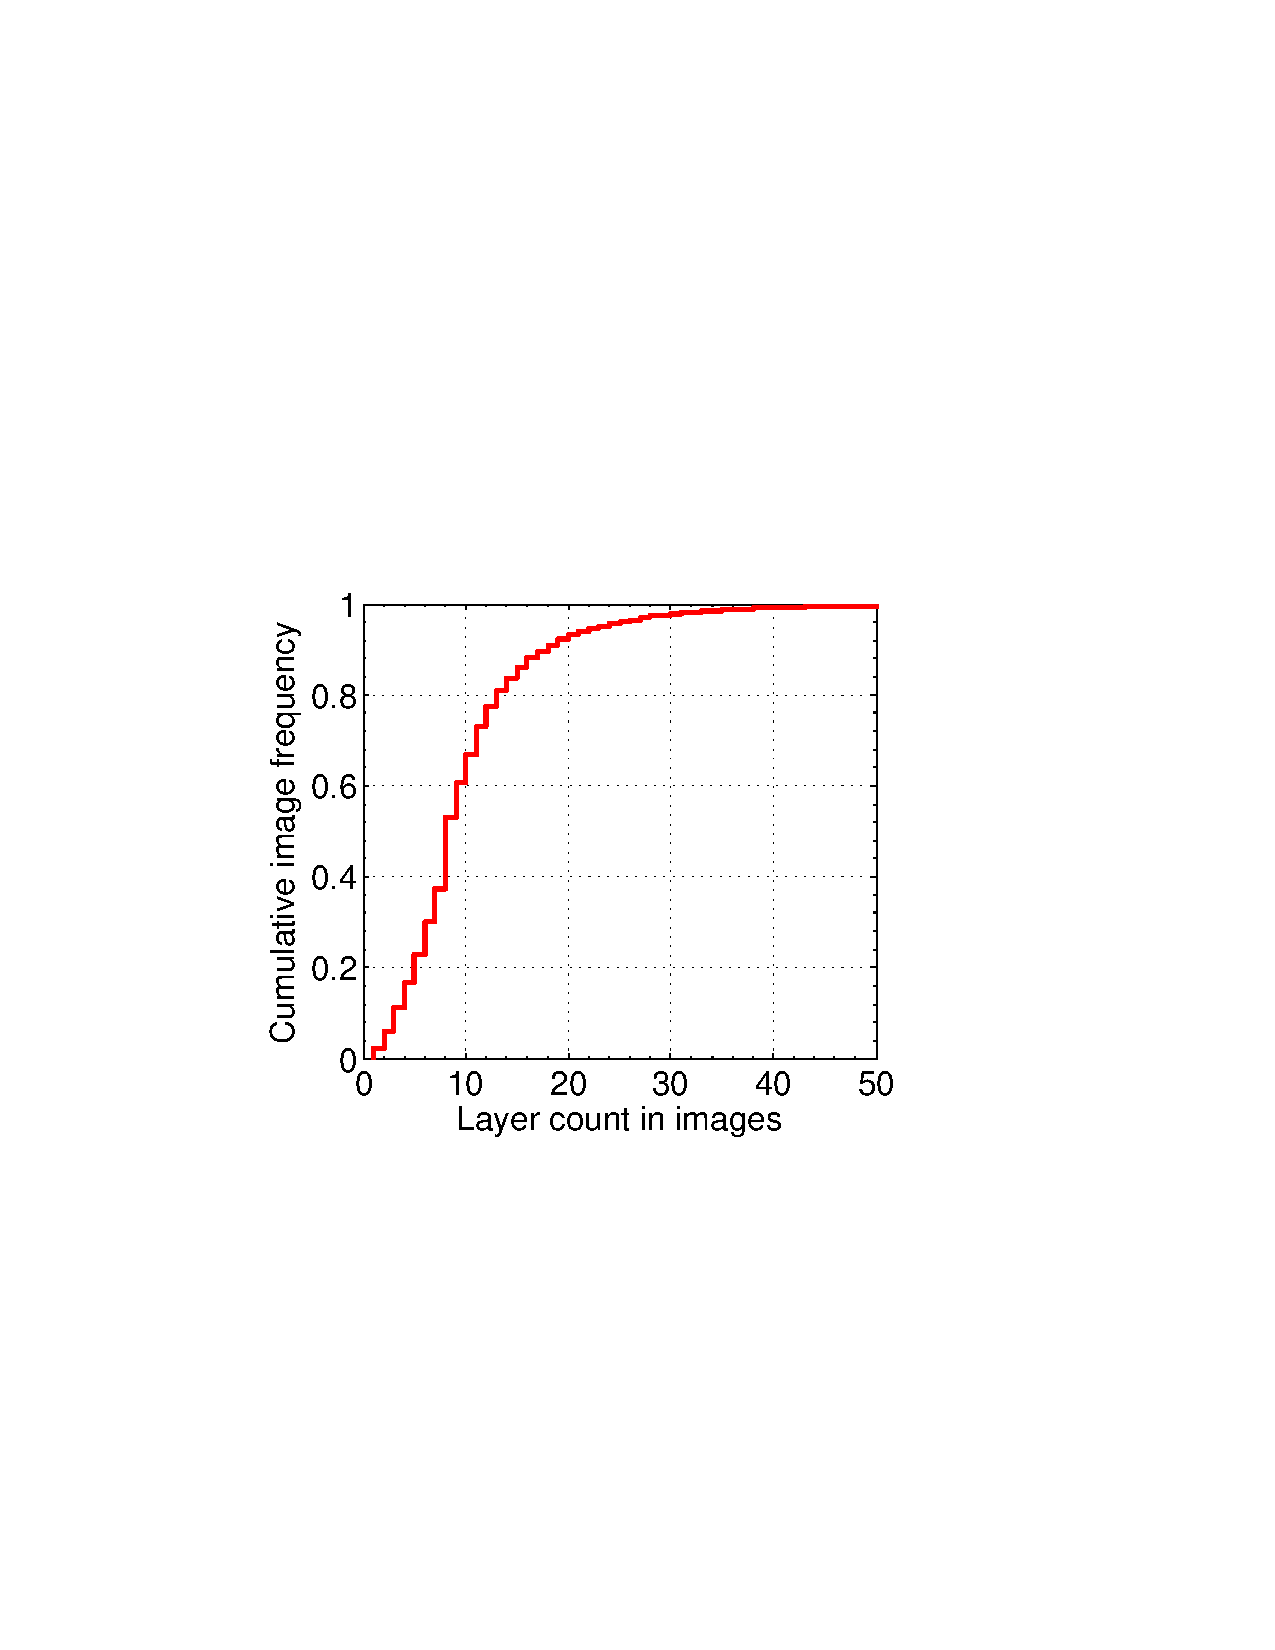
\includegraphics[width=0.23\textwidth]{graphs/layer_cnt_less.pdf}
	}
	\subfigure[Histogram of images by Layer count in images]{\label{fig_hist_layer_cnt}
		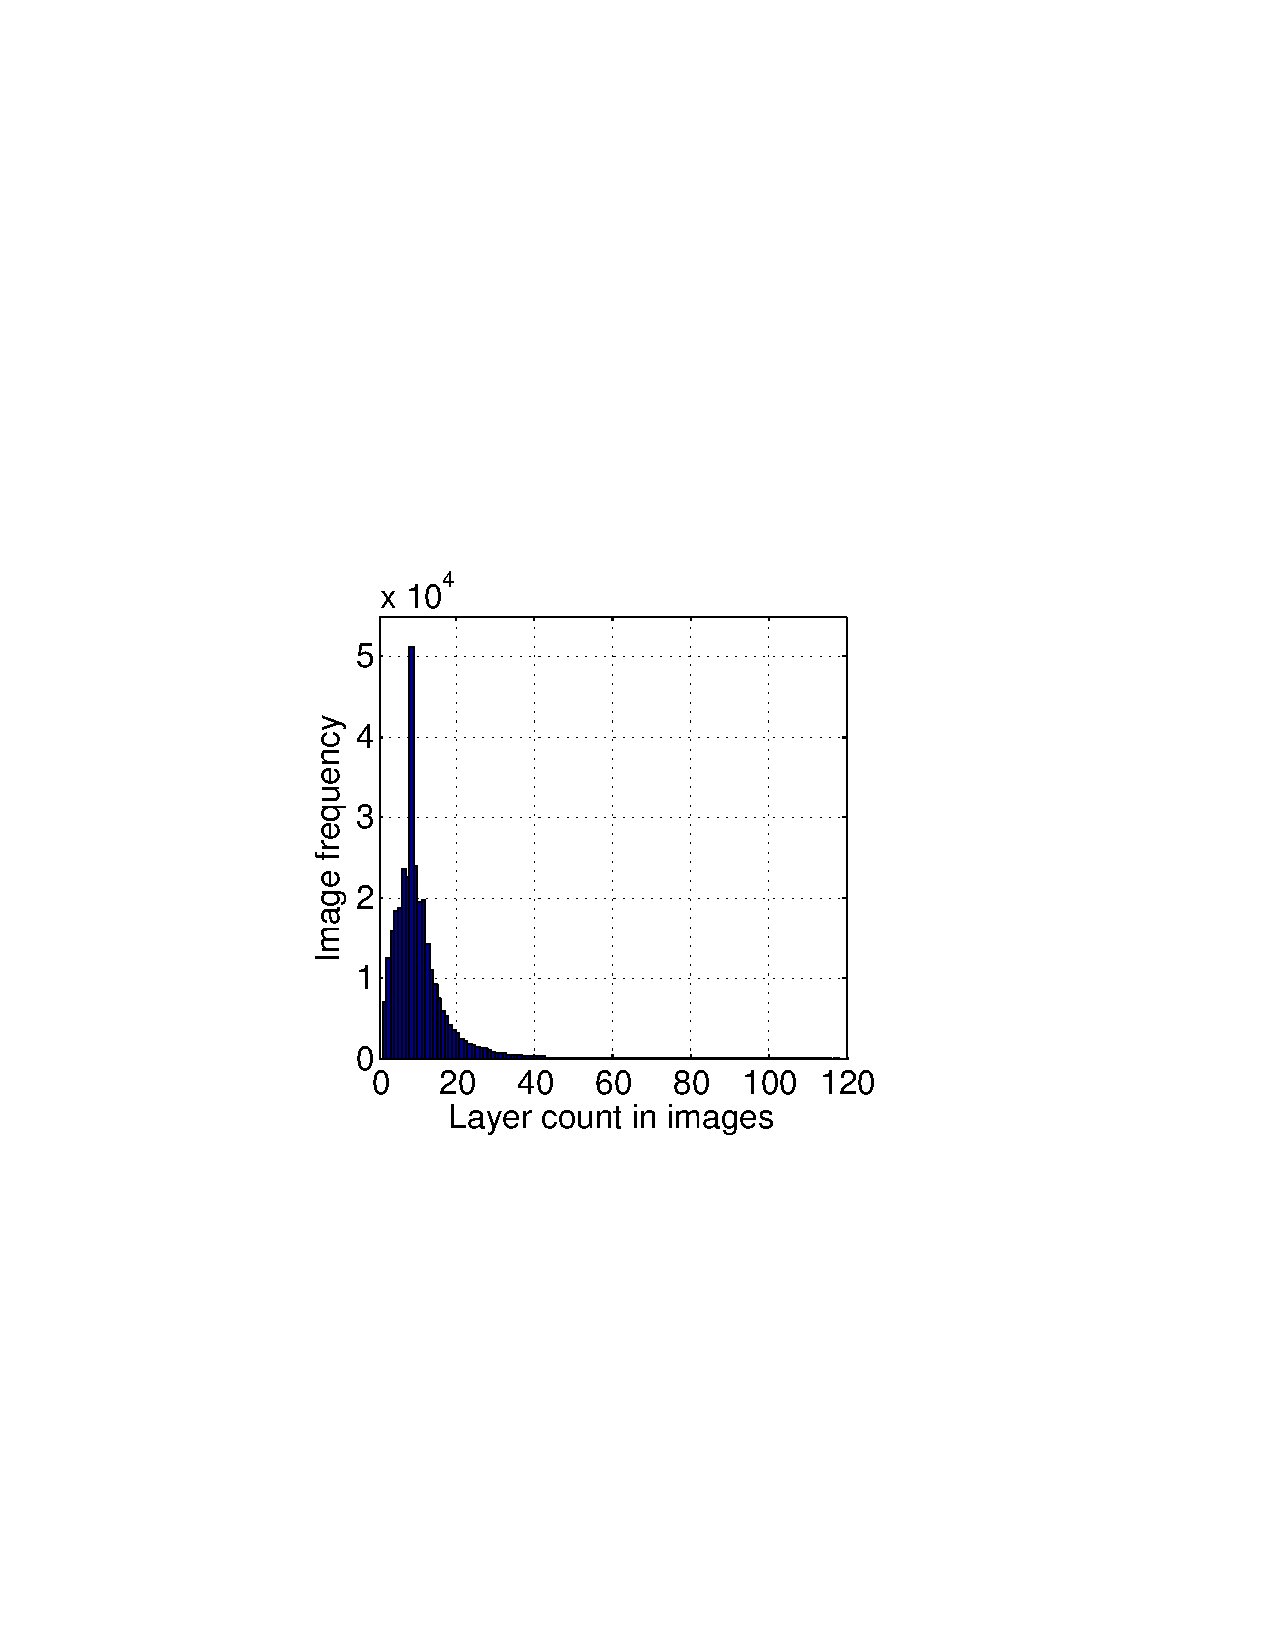
\includegraphics[width=0.213\textwidth]{graphs/hist_layer_cnt.pdf}
	}
	\caption{Compression rate distribution}
	\label{fig-layer-cnt}
\end{figure}

As discussed in~\ref{sec-image-layers}, images are consisted of a set of layers. Figure~\ref{fig-layer-cnt} shows the cumulative image frequency by layer count in images. 90\% of images have less than 18 layers. Half of images have less than 8 layers. 

Figure~\ref{fig_hist_layer_cnt} shows the histogram of images by layer count in images. About 51,300 images have 8 layers, which is the peak value in the figure. The maximum layer count is 121. The average is 10. 7,060 images have only 1 layer. 

\begin{figure}[!t]
	\centering
	\subfigure[CDF of layer by layer count]{\label{fig_repeate_layer}
		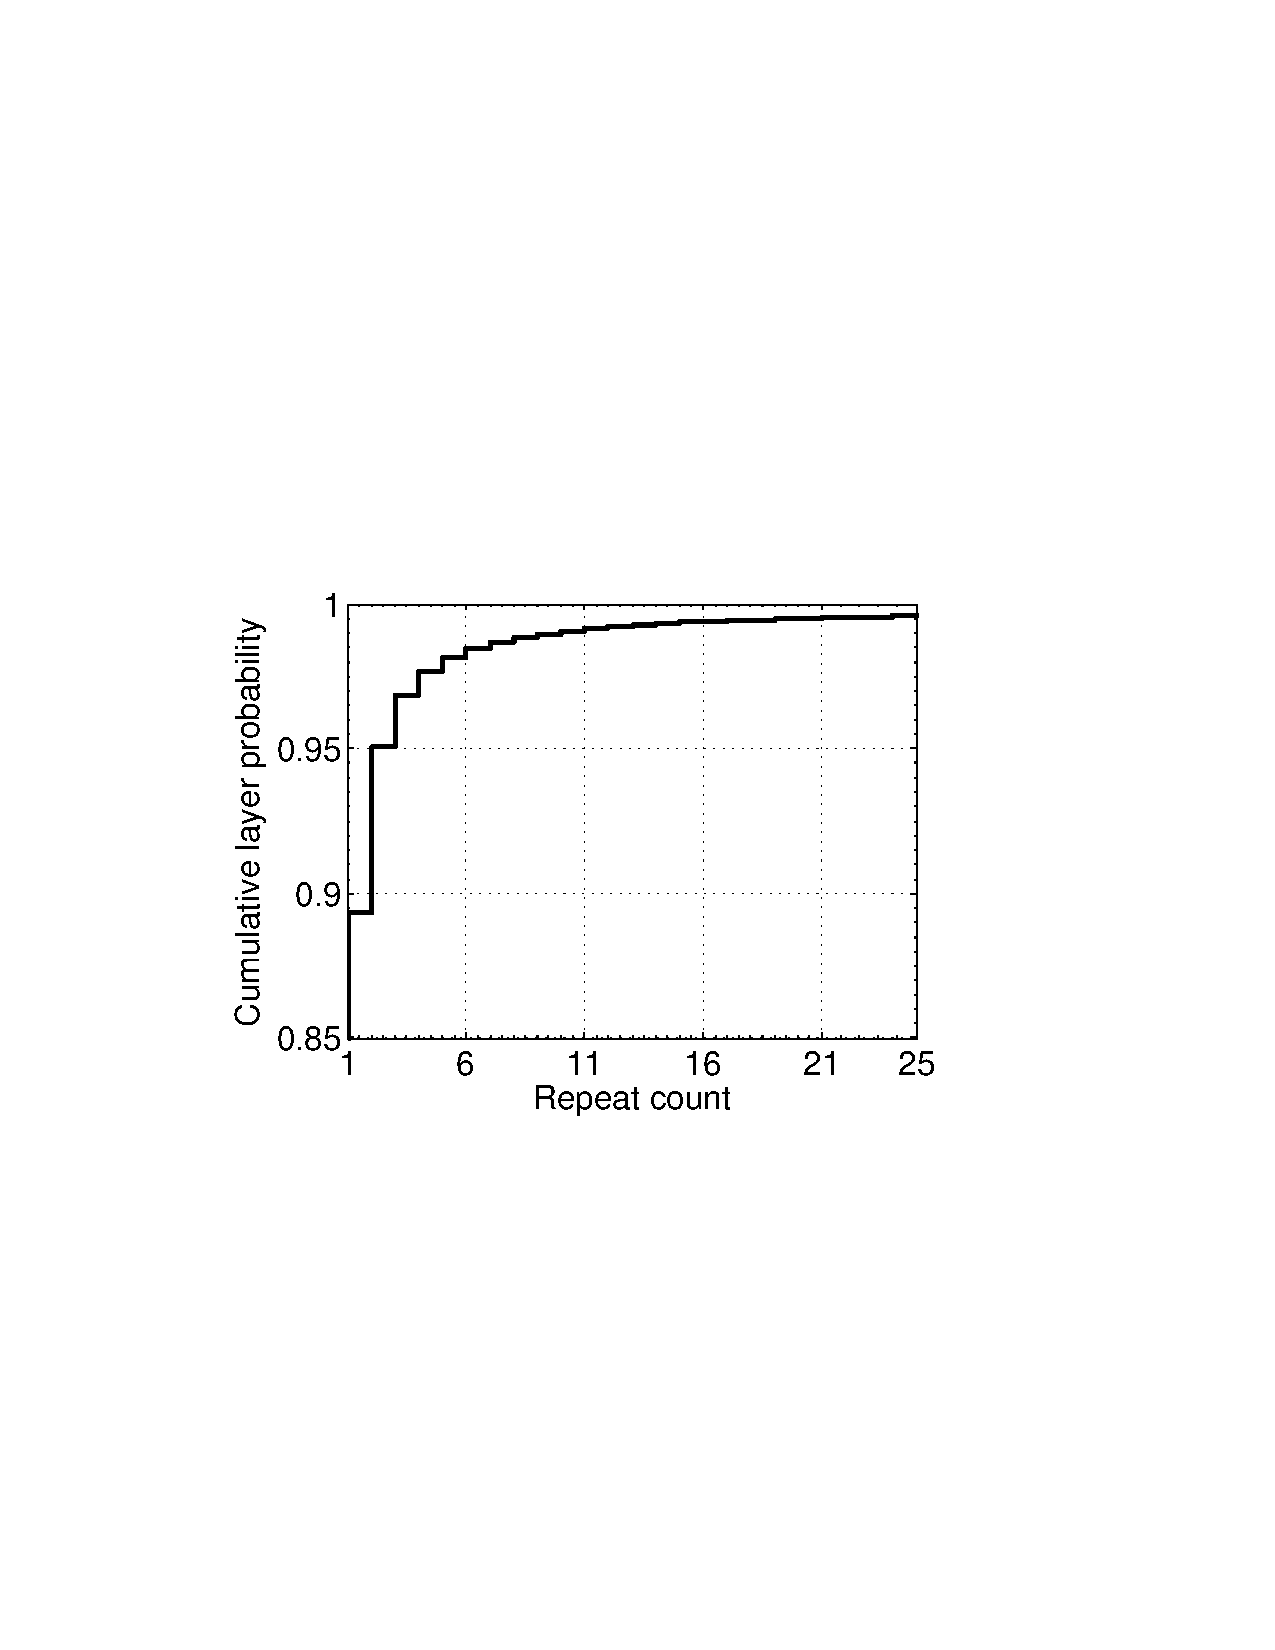
\includegraphics[width=0.23\textwidth]{graphs/repeate_layer.pdf}
	}
	\subfigure[Histogram of images by layer count in images]{\label{fig_hist_repeate_layer}
		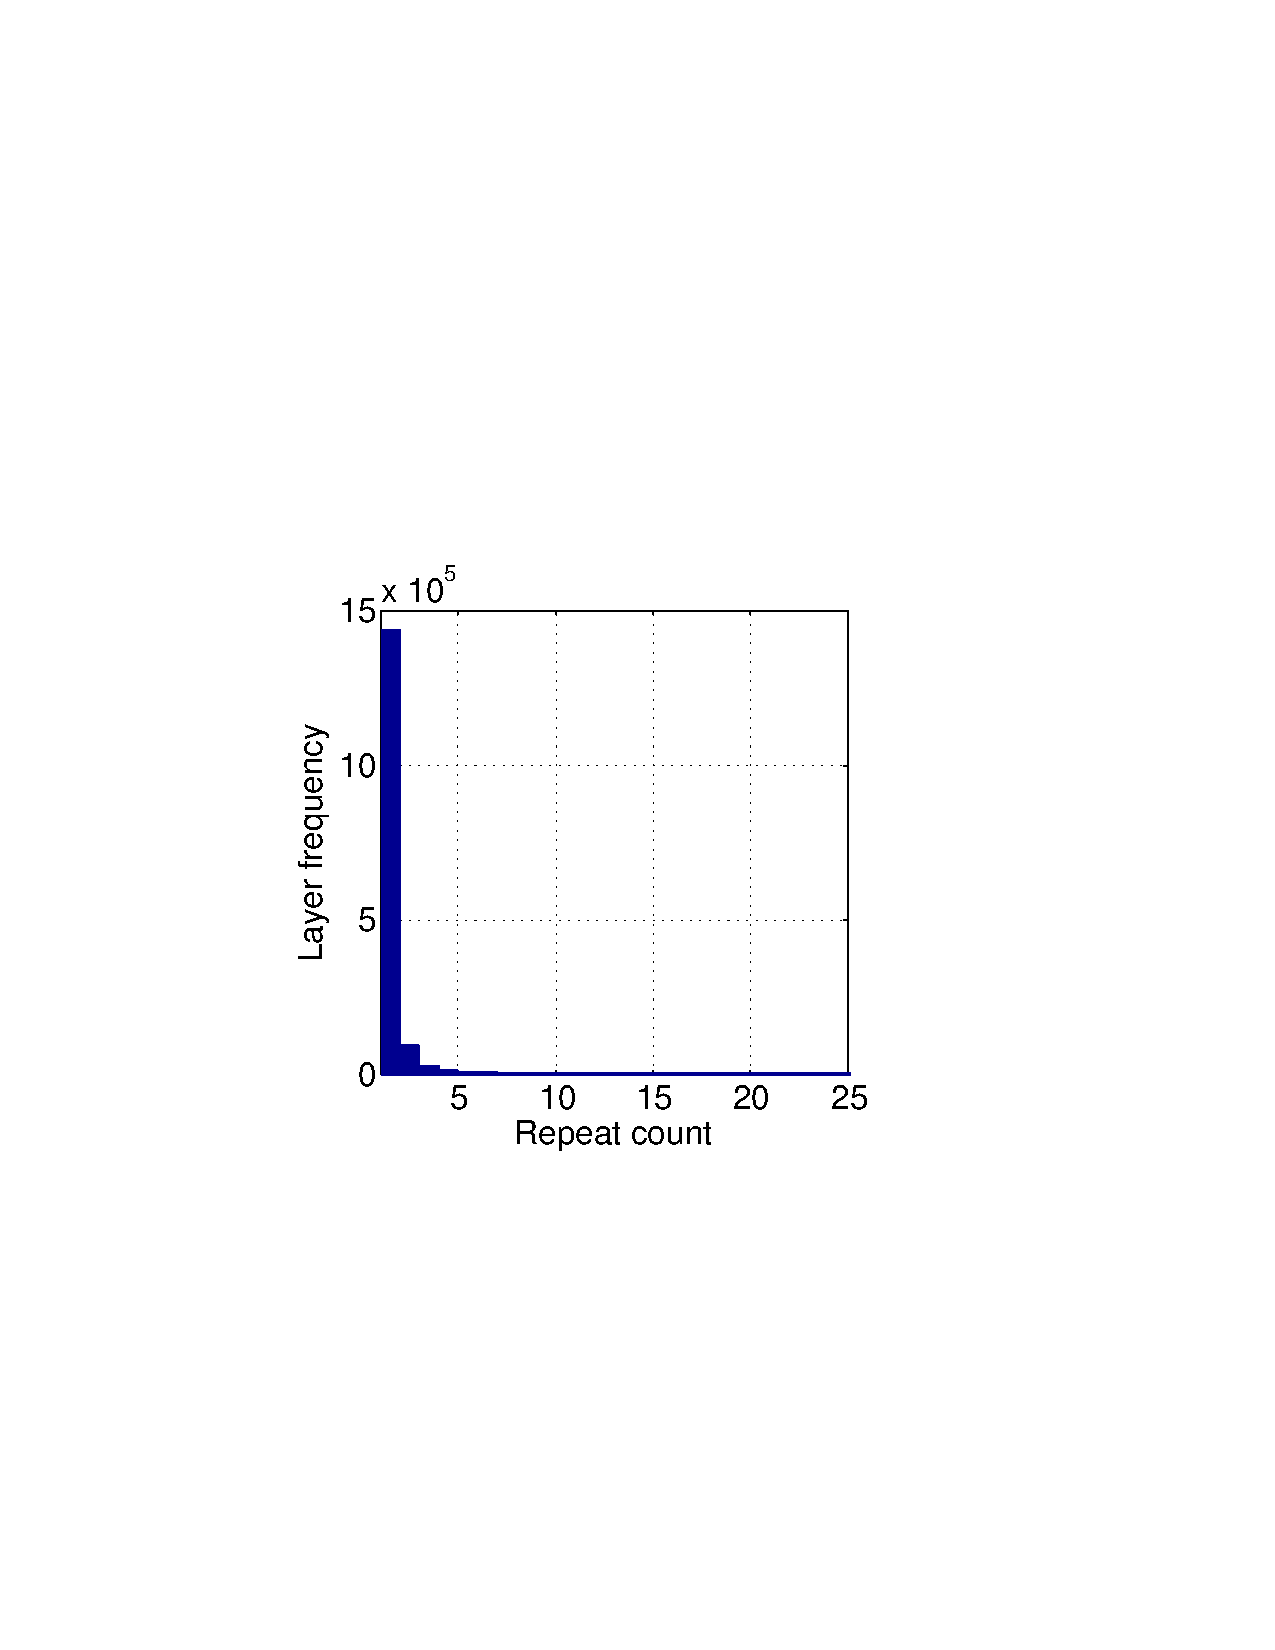
\includegraphics[width=0.223\textwidth]{graphs/hist_repeate_layer.pdf}
	}
	\caption{Compression rate distribution}
	\label{fig-repeat-layer-cnt}
\end{figure}

\subsubsection{Repeat layer count distribution}

As discussed in~\ref{sec-image-layers}, layers are shared among images. Figure~\ref{fig_repeate_layer} shows the cumulative layer frequency by repeat count among images. Around 90\% of layers are only reference by a single image. 99\% of layers are shared among less than 25 images. 

Figure~\ref{fig_hist_repeate_layer} shows the histogram of layers by repeat count among images. About 1,440,000 layers are referenced by only one single image, which is the peak value in the figure. The maximum repeat count is 33,428 while the median is 1. The average is 2.

\subsubsection{Directory count distribution}

\begin{figure}
	\centering
	\begin{minipage}{0.27\textwidth}
		\centering
		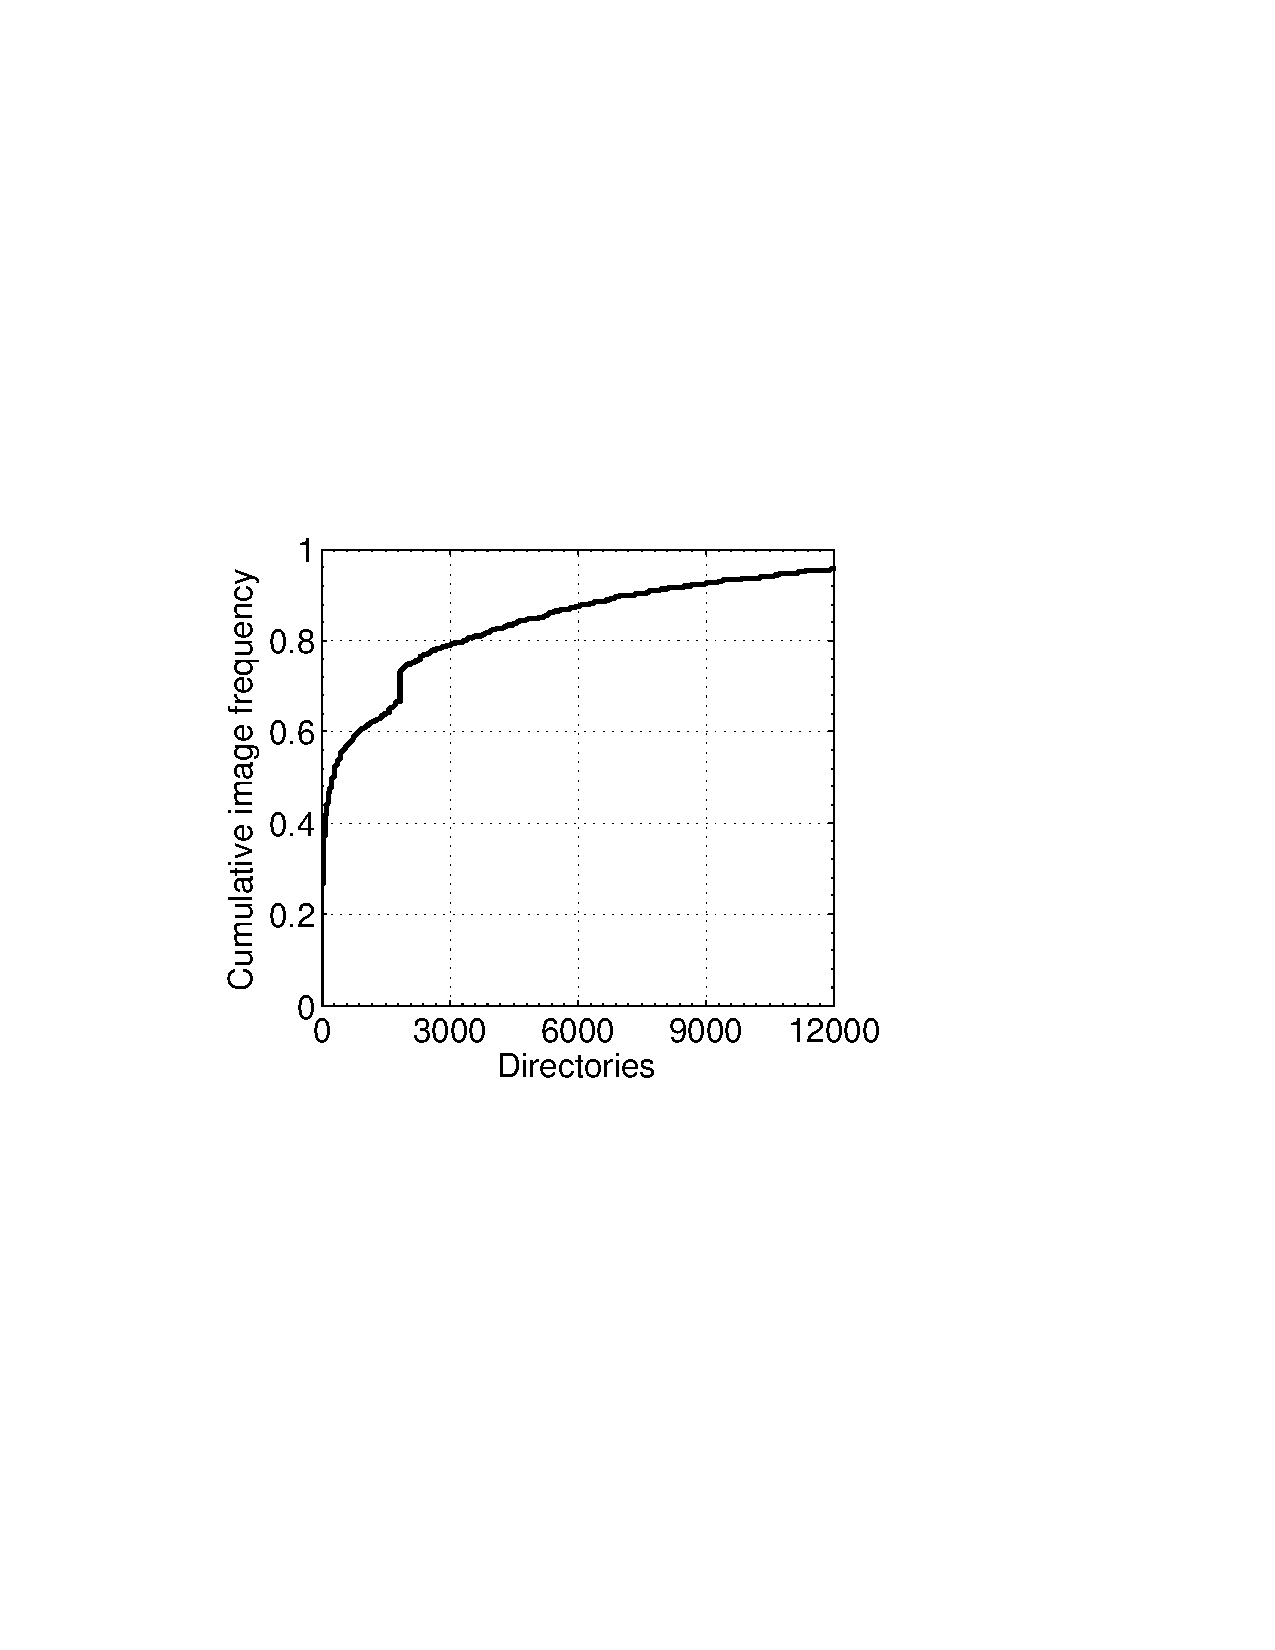
\includegraphics[width=1\textwidth]{graphs/dir.pdf}
		\caption{CDF of images by directories}
		\label{fig-dir}
	\end{minipage}%
	\begin{minipage}{0.23\textwidth}
		\centering
		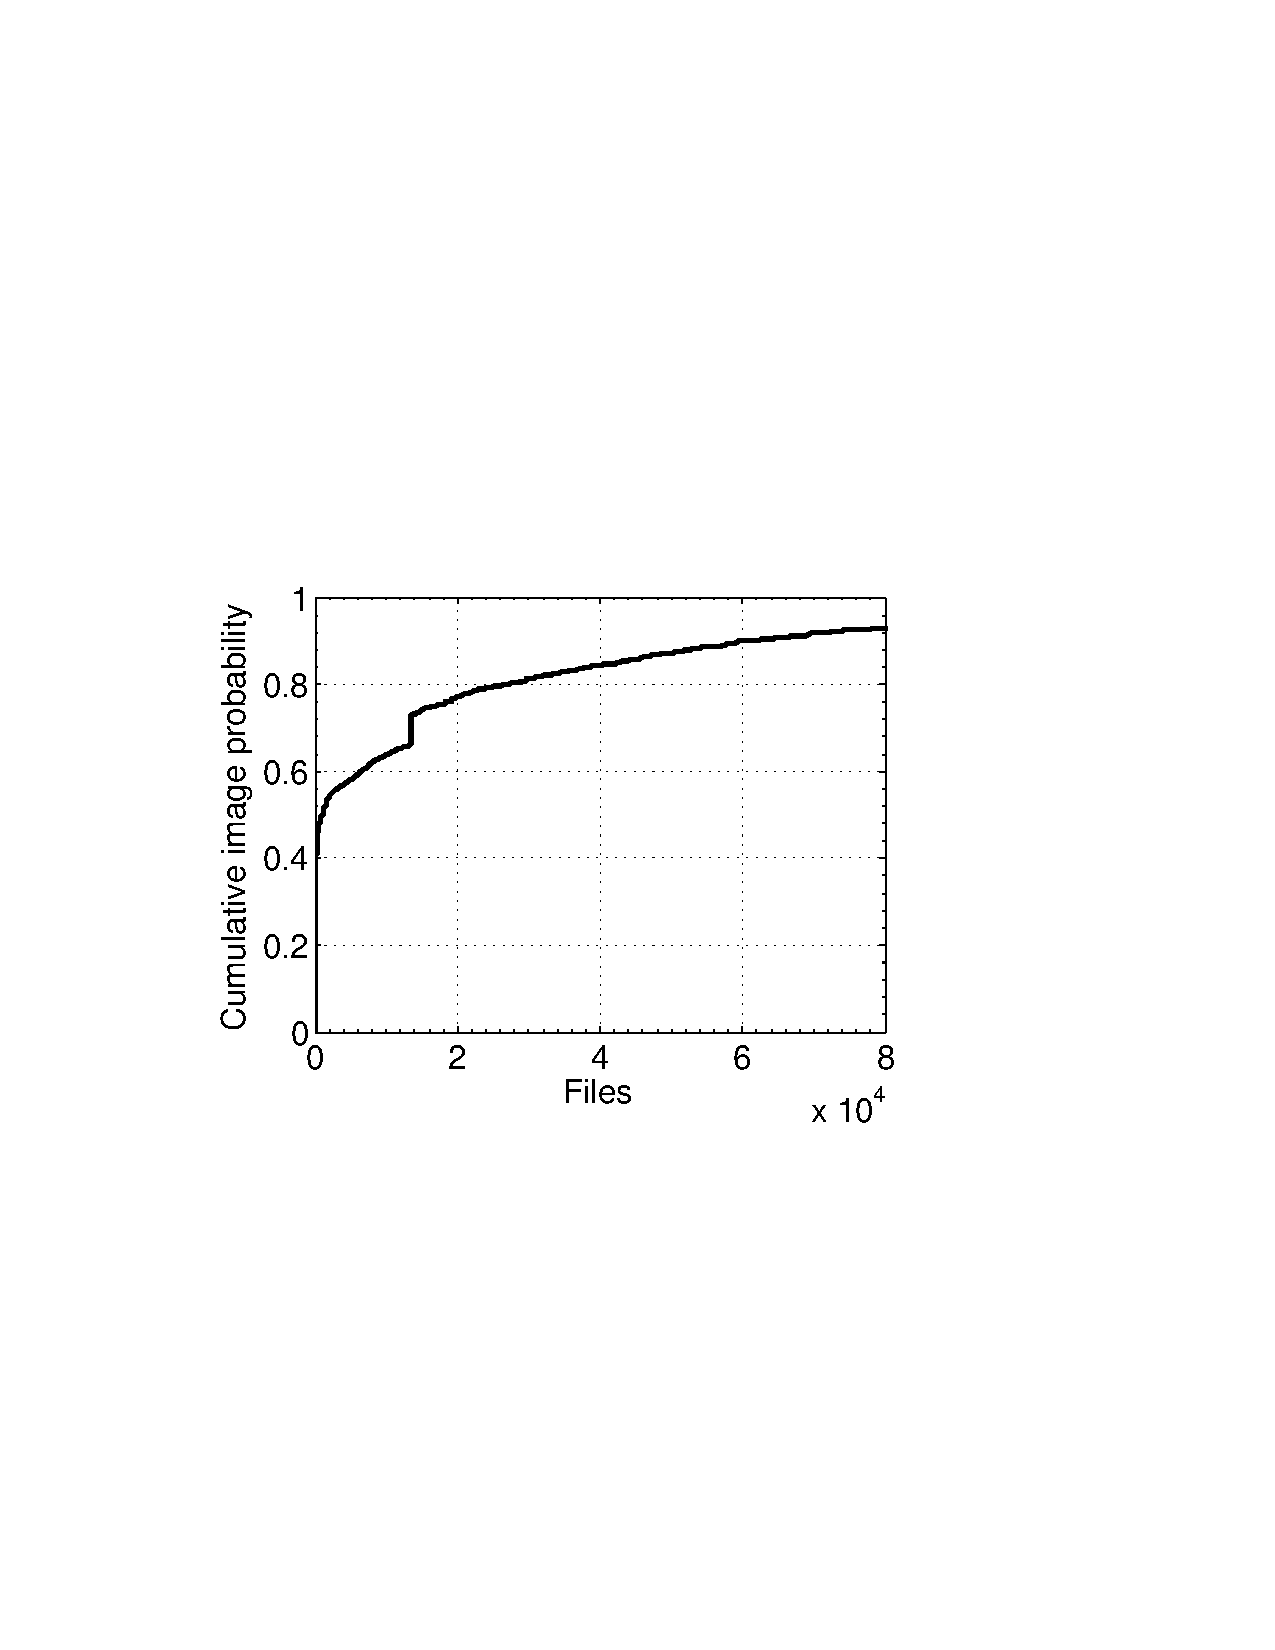
\includegraphics[width=1\textwidth]{graphs/file.pdf}
		\caption{CDF of images by files}
		\label{fig-file}
	\end{minipage}
\end{figure}

Figure~\ref{fig-dir} shows the cumulative image frequency by directories. 90\% of images have less than 7,344 directories. Half of images have less than 296 directories. The maximum is 1,168,160 while the minimum is 1. The average is 2705. 

\subsubsection{File count distribution}

Figure~\ref{fig-file} shows the cumulative image frequency by files. 90\% of images have less than 64,780 files. Half of images have less than 1,090 files. The maximum is 8,509,958 while the minimum is 1. The average is 21,413. 

\subsection{Layer}

\subsubsection{Layer size distribution}

\begin{figure}[!t]
	\centering
	\subfigure[CDF of layers by layer size]{\label{fig_layer_size_cdf}
		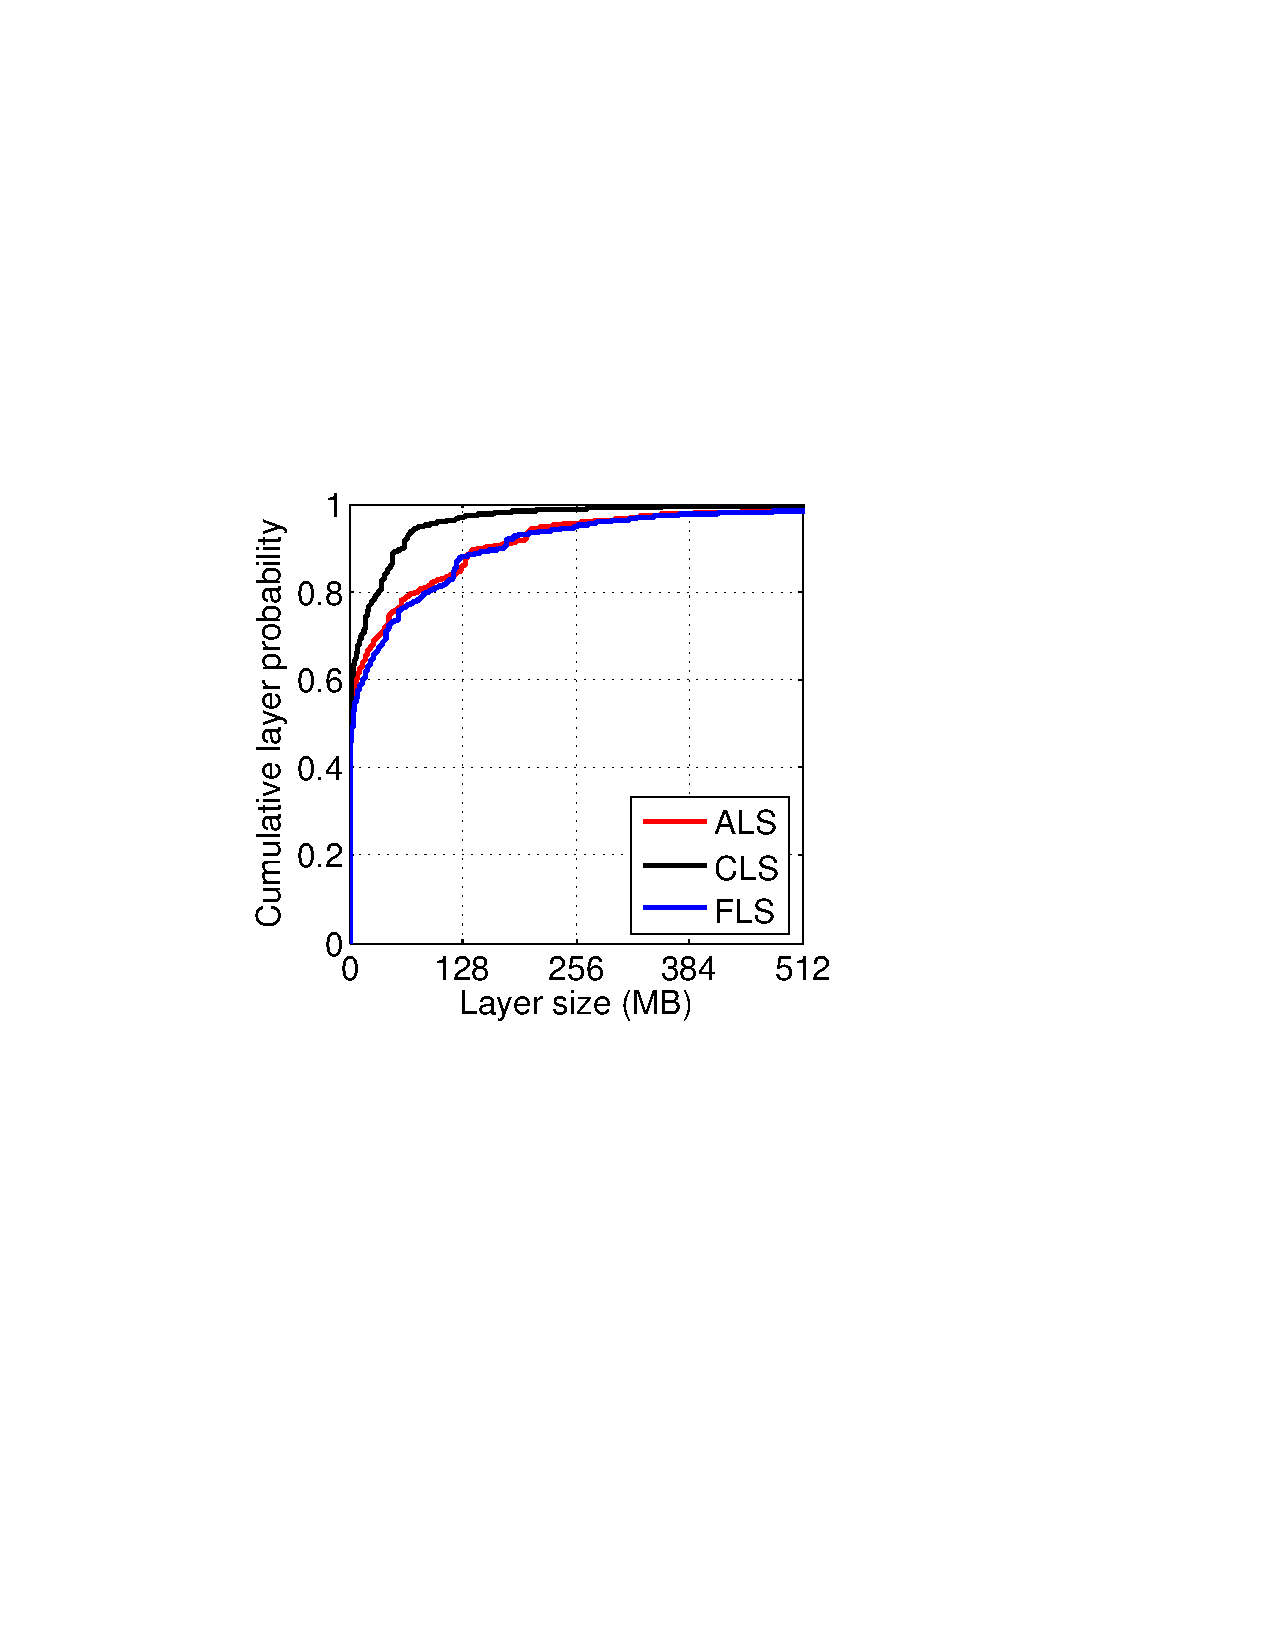
\includegraphics[width=0.23\textwidth]{graphs/layer_size_mb.pdf}
	}
	\subfigure[Histogram of layers by layer size]{\label{fig_hist_layer_size}
		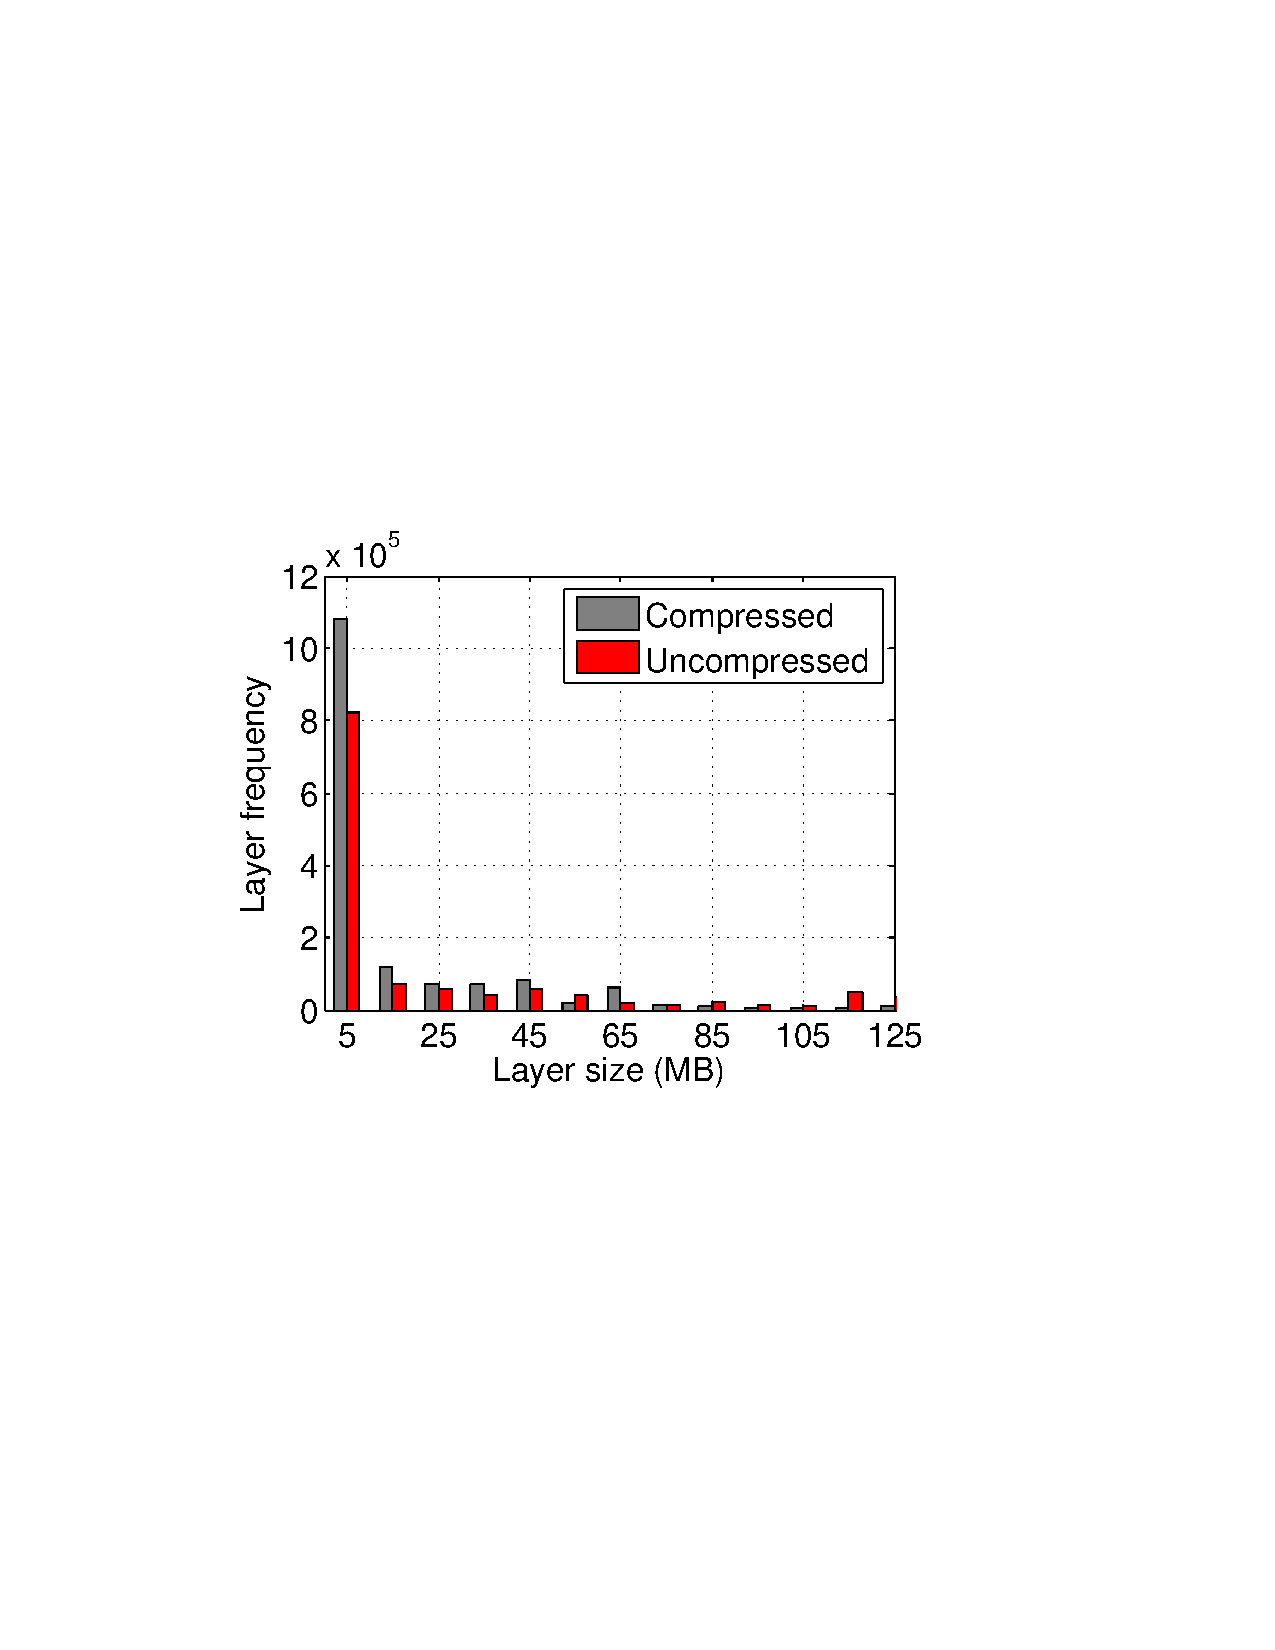
\includegraphics[width=0.223\textwidth]{graphs/hist_layer_size.pdf}
	}
	\caption{Layer size distribution}
	\label{fig-layer-size}
\end{figure}

Like image size, we also measured three kinds of layer size: archival size, compression size, and the sum of containing file size. Compression size is the original layer size after downloaded; The archival size is the decompressed layer size without extracting and unpacking; The sum of containing file size is the sum of its containing file size after decompression with extracting and unpacking.

Figure~\ref{fig_layer_size_cdf} shows the cumulative layer probability by layer size for three kinds of layer size.
As shown in figure~\ref{fig_layer_size_cdf}, the red curve and blue curve are almost overlapped, which means that the distribution of archival size and the distribution of sum of file size are similar. 90\% of layers have a less than 177 MB uncompression size (i.e., archival size or the sum of containing file size), while 90\% of layers have a less than 63 MB compression size. Half of layers are less than ~4 MB (i.e., uncompression size or compression size). The largest uncompression image size is ~29 GB (23 GB for the sum of file size) while the largest compression size is only 19 GB.
Figure~\ref{fig_hist_layer_size} shows the histogram of layer by layer size. About 1,080,000 of the layers' compression size is less than 5 MB while 985,000 layers' archival size less than 5 MB, 820,000 layers' sum of file size is less than 5 MB. 
Figure~\ref{fig-layer-size} shows that the majority of the layers in Docker hub have a smaller size. 90\% of layer can be compressed with less than 63 MB and 77\% of images are less than 63 MB even without compression. 

\subsubsection{Layer compression ratio distribution}

\begin{figure}[!t]
	\centering
	\subfigure[CDF of layers by layer size]{\label{fig_cdf_compression_ratio}
		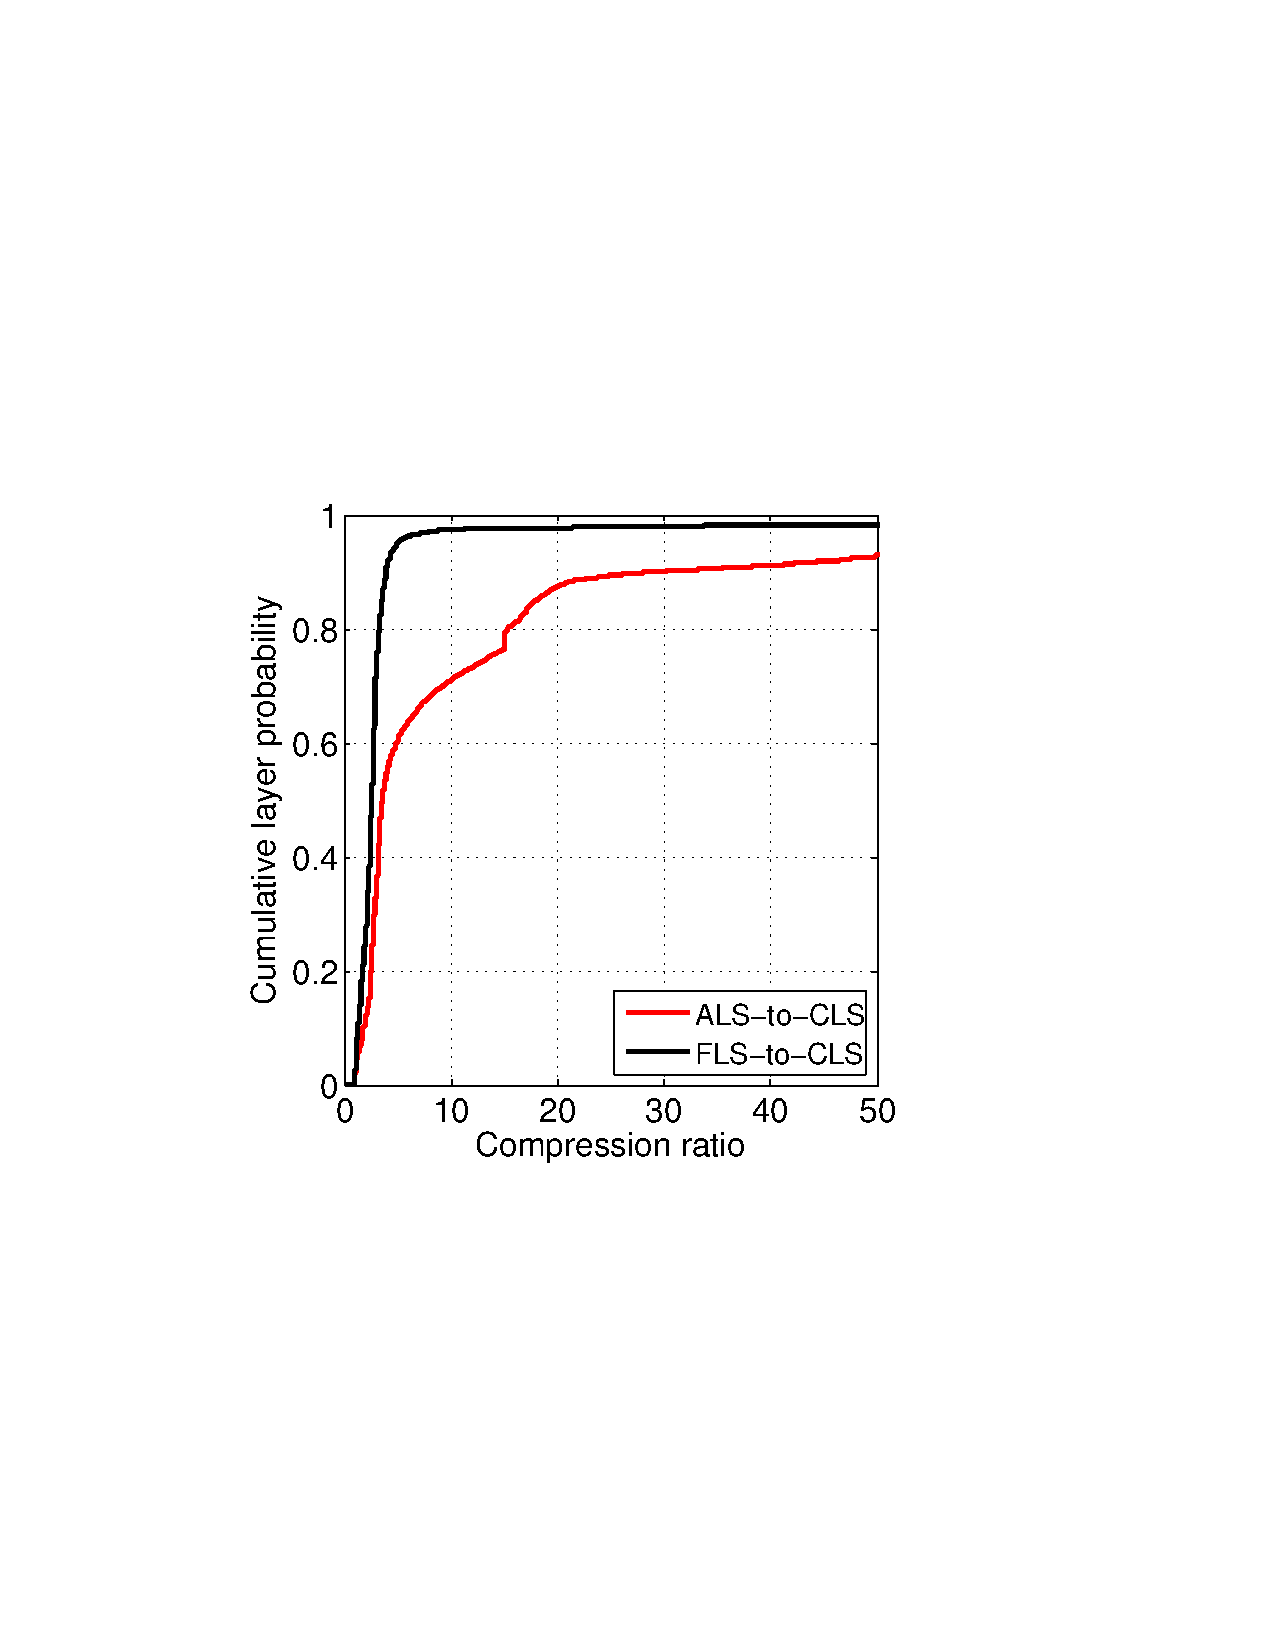
\includegraphics[width=0.23\textwidth]{graphs/cdf_compression_ratio.pdf}
	}
	\subfigure[Histogram of layers by layer size]{\label{fig_his_compression_ratio}
		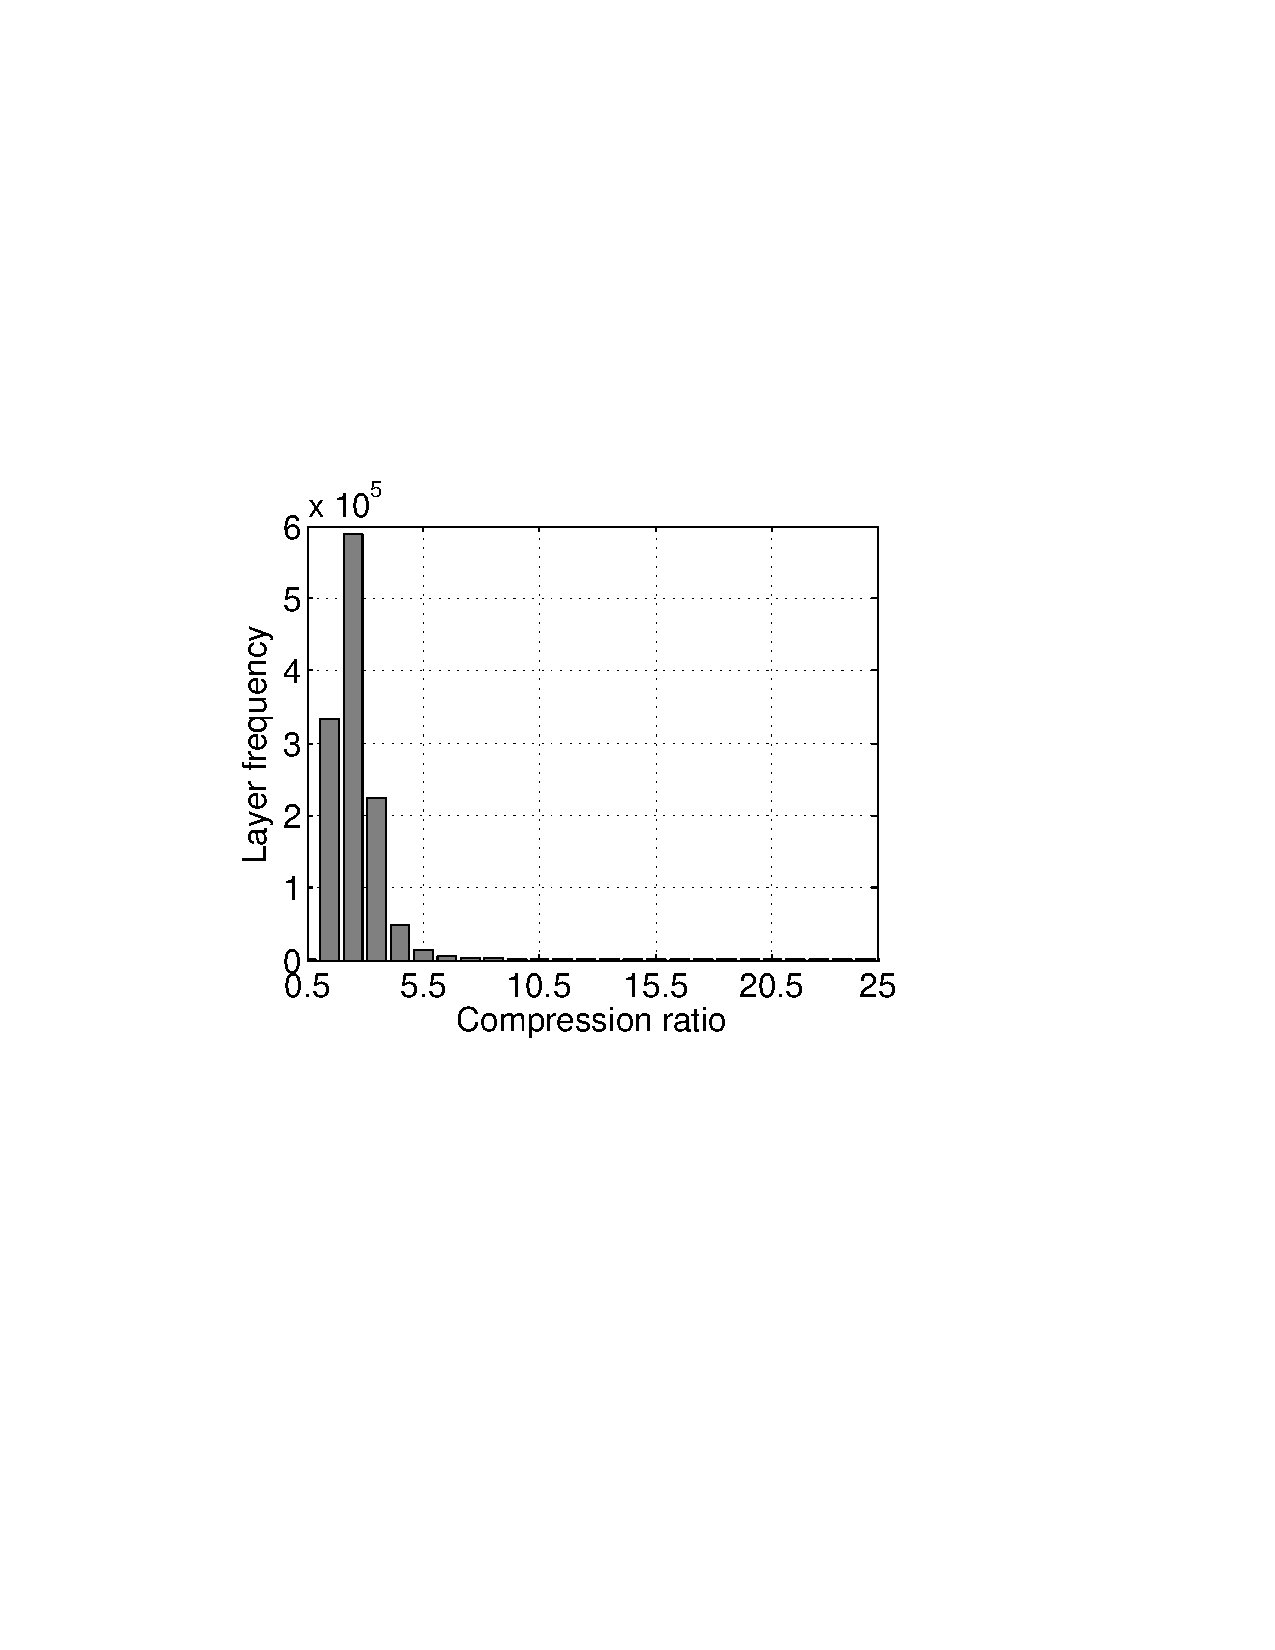
\includegraphics[width=0.223\textwidth]{graphs/his_compression_ratio.pdf}
	}
	\caption{Layer compression ratio distribution}
	\label{fig-compression-ratio}
\end{figure}

Since three kinds of layer size are measured: archival size, compression size, and the sum of containing file size. Thus, we calculated two kinds of compression ratio: the ratio of archival size to compression size and the ratio of Sum of file size to compression size. 

Figure~\ref{fig_cdf_compression_ratio} shows the cumulative layer probability by compression ratio. Overall, we can see that the ratio of archival size to compression size is greater than the ratio of the sum of file size to the compression size. 90\% of images have a archival-to-compression ratio less than ~4 while 90\% of images have a sum of file-to-compression ratio less than 30. Half of the images have a compression ratio (both archival-to-compression and sum of files-to-compression) around 3. The maximum compression ratio are 512,930 and 1026 for the ratio of sum to file size to compression size and the ratio of archival to compression size respectively.
Figure~\ref{fig_his_compression_ratio} shows a histogram of layer by compression ratio. 587,000 images have a ratio of sum of file size to compression size of 3 and 331,000 images have a ratio of archival size to compression size of 3, which are two peaks shown in the graph.

Figure~\ref{fig-compression-ratio} suggests that layers have a great potential for compression to save space.

\subsubsection{Layer depth distribution}

After extracting and unpacking gzip compressed layer archival files, we calculated the layer directory depth (i.e., the maximum directory depth). 
Figure~\ref{fig_layer_depth} shows the cumulative layer probability by layer directory depth. Around 90\% of layers' directory depth is less than 10. 50\% of layers' directory depth is less than 4. 

Figure~\ref{fig_hist_layer_depth} shows the histogram of layers by layer directory depth. About 313,000 layers' layer directory depth is 3, which is the peak value in the figure. The maximum repeat count is 444 while the median is 4. The average is ~5.

\begin{figure}[!t]
	\centering
	\subfigure[CDF of layers by layer directory depth]{\label{fig_layer_depth}
		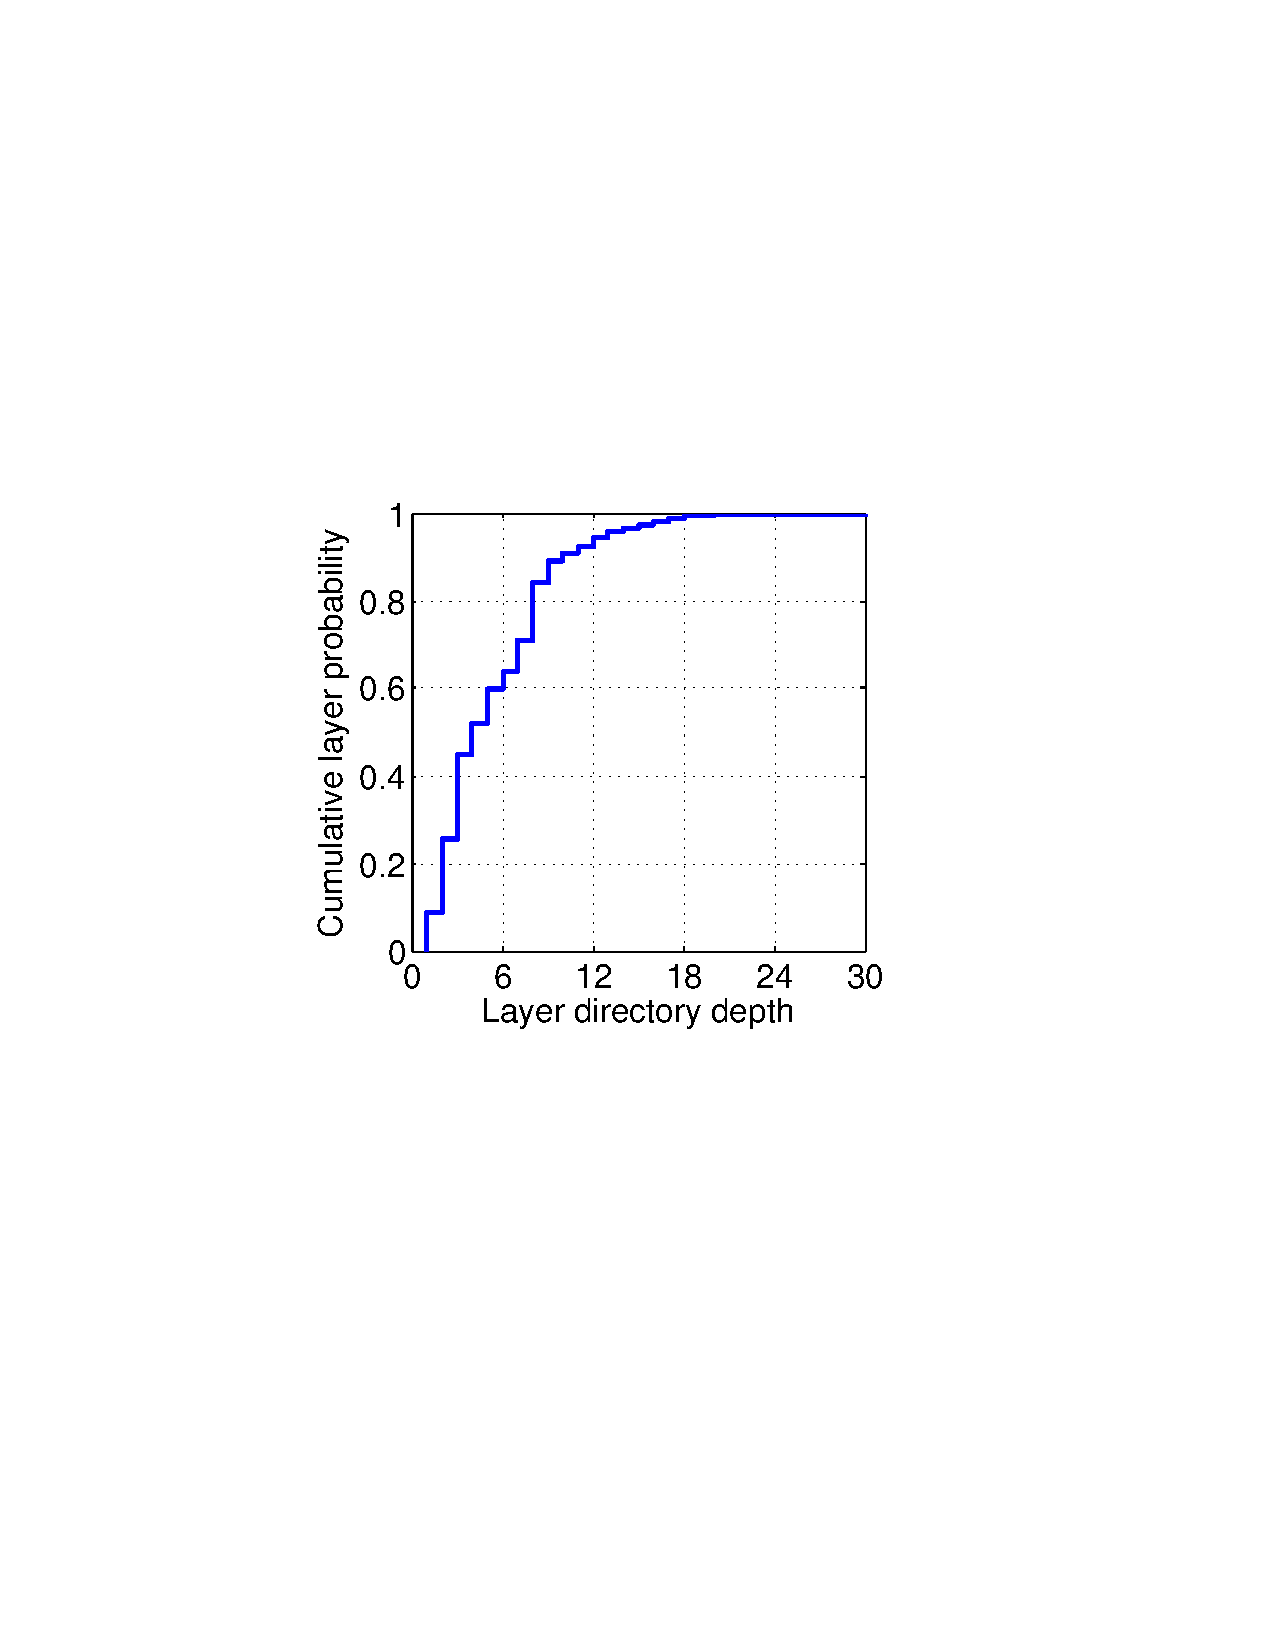
\includegraphics[width=0.23\textwidth]{graphs/layer_depth.pdf}
	}
	\subfigure[Histogram of layers by layer directory depth]{\label{fig_hist_layer_depth}
		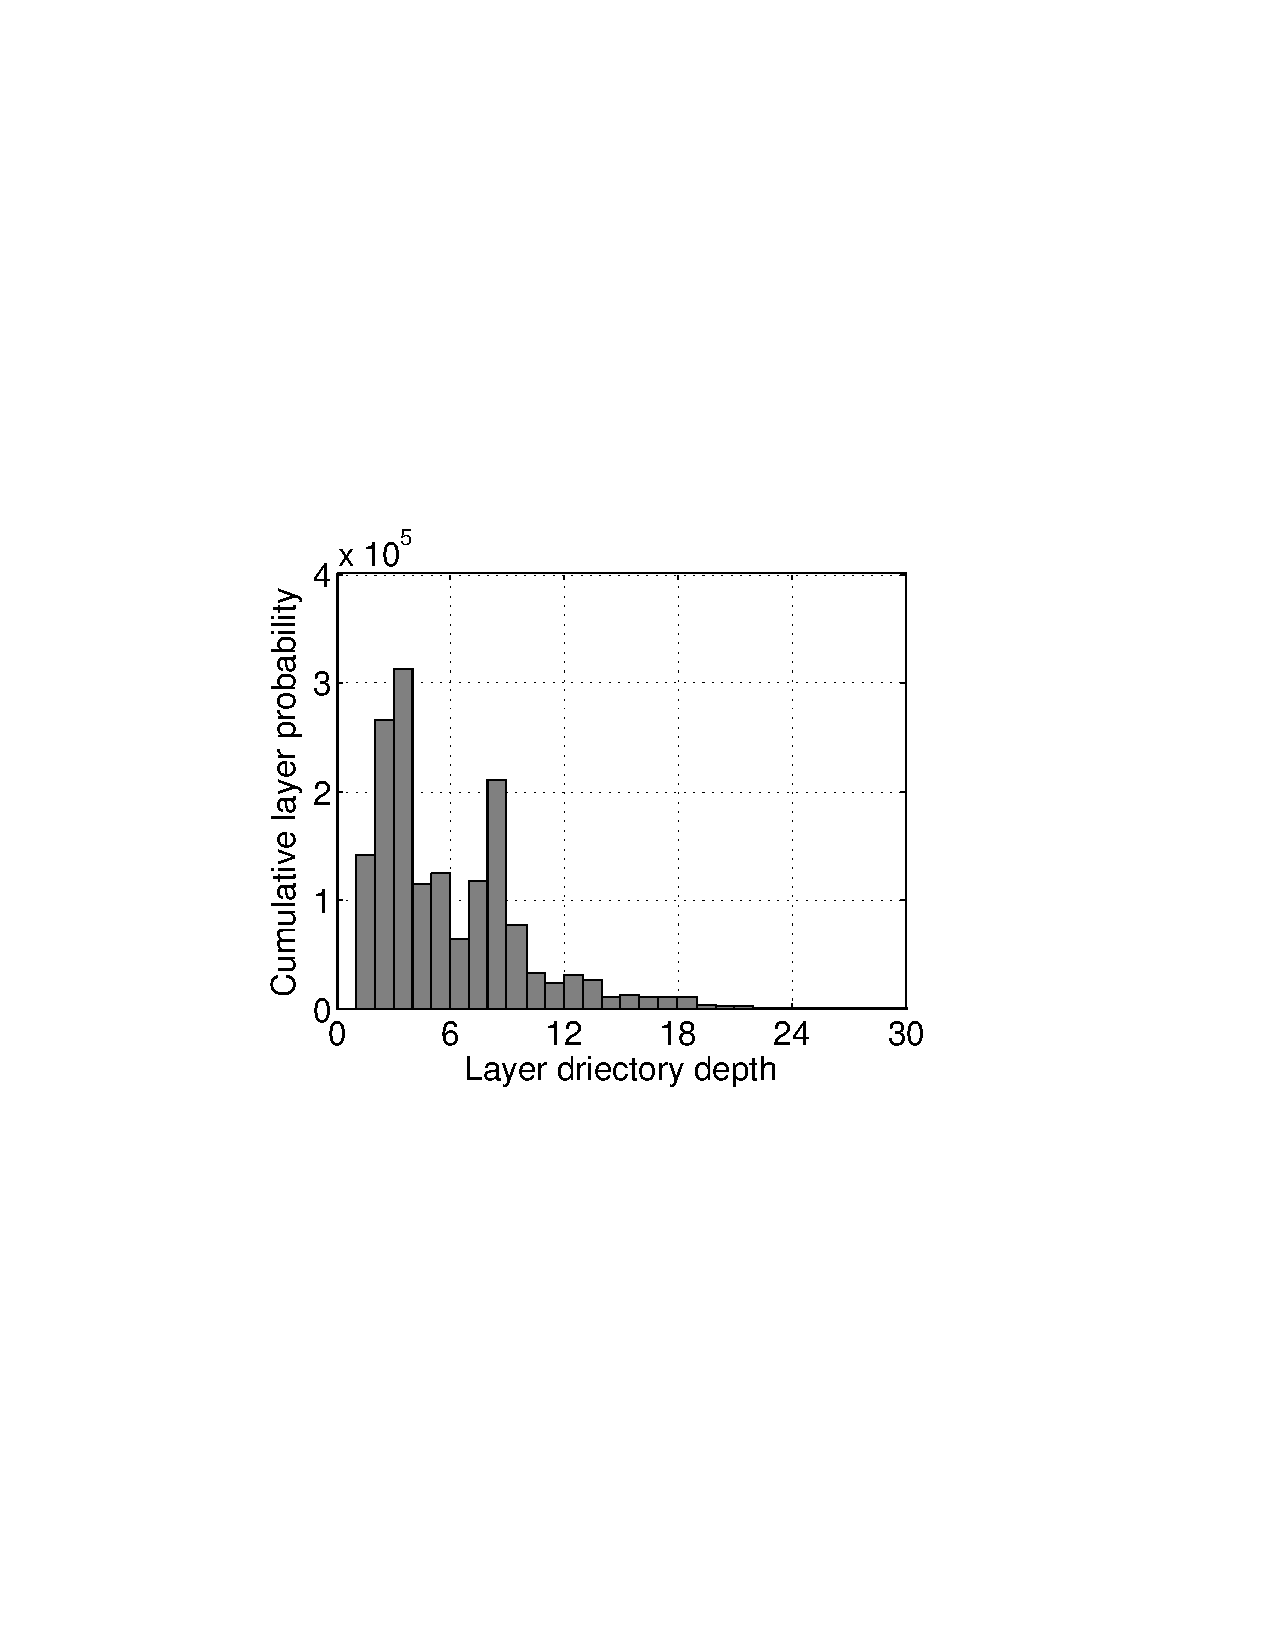
\includegraphics[width=0.22\textwidth]{graphs/hist_layer_depth.pdf}
	}
	\caption{Layer directory depth distribution}
	\label{fig-layer-dir}
\end{figure}

\subsubsection{Directory count distribution}

Figure~\ref{fig_dir_cnt} shows the cumulative layer probability by directories. 90\% of images have less than 826 directories. Half of images have less than 11 directories. The maximum is 111,940 while the minimum is 1. The average is 273. 

\begin{figure}
	\centering
	\begin{minipage}{0.25\textwidth}
		\centering
		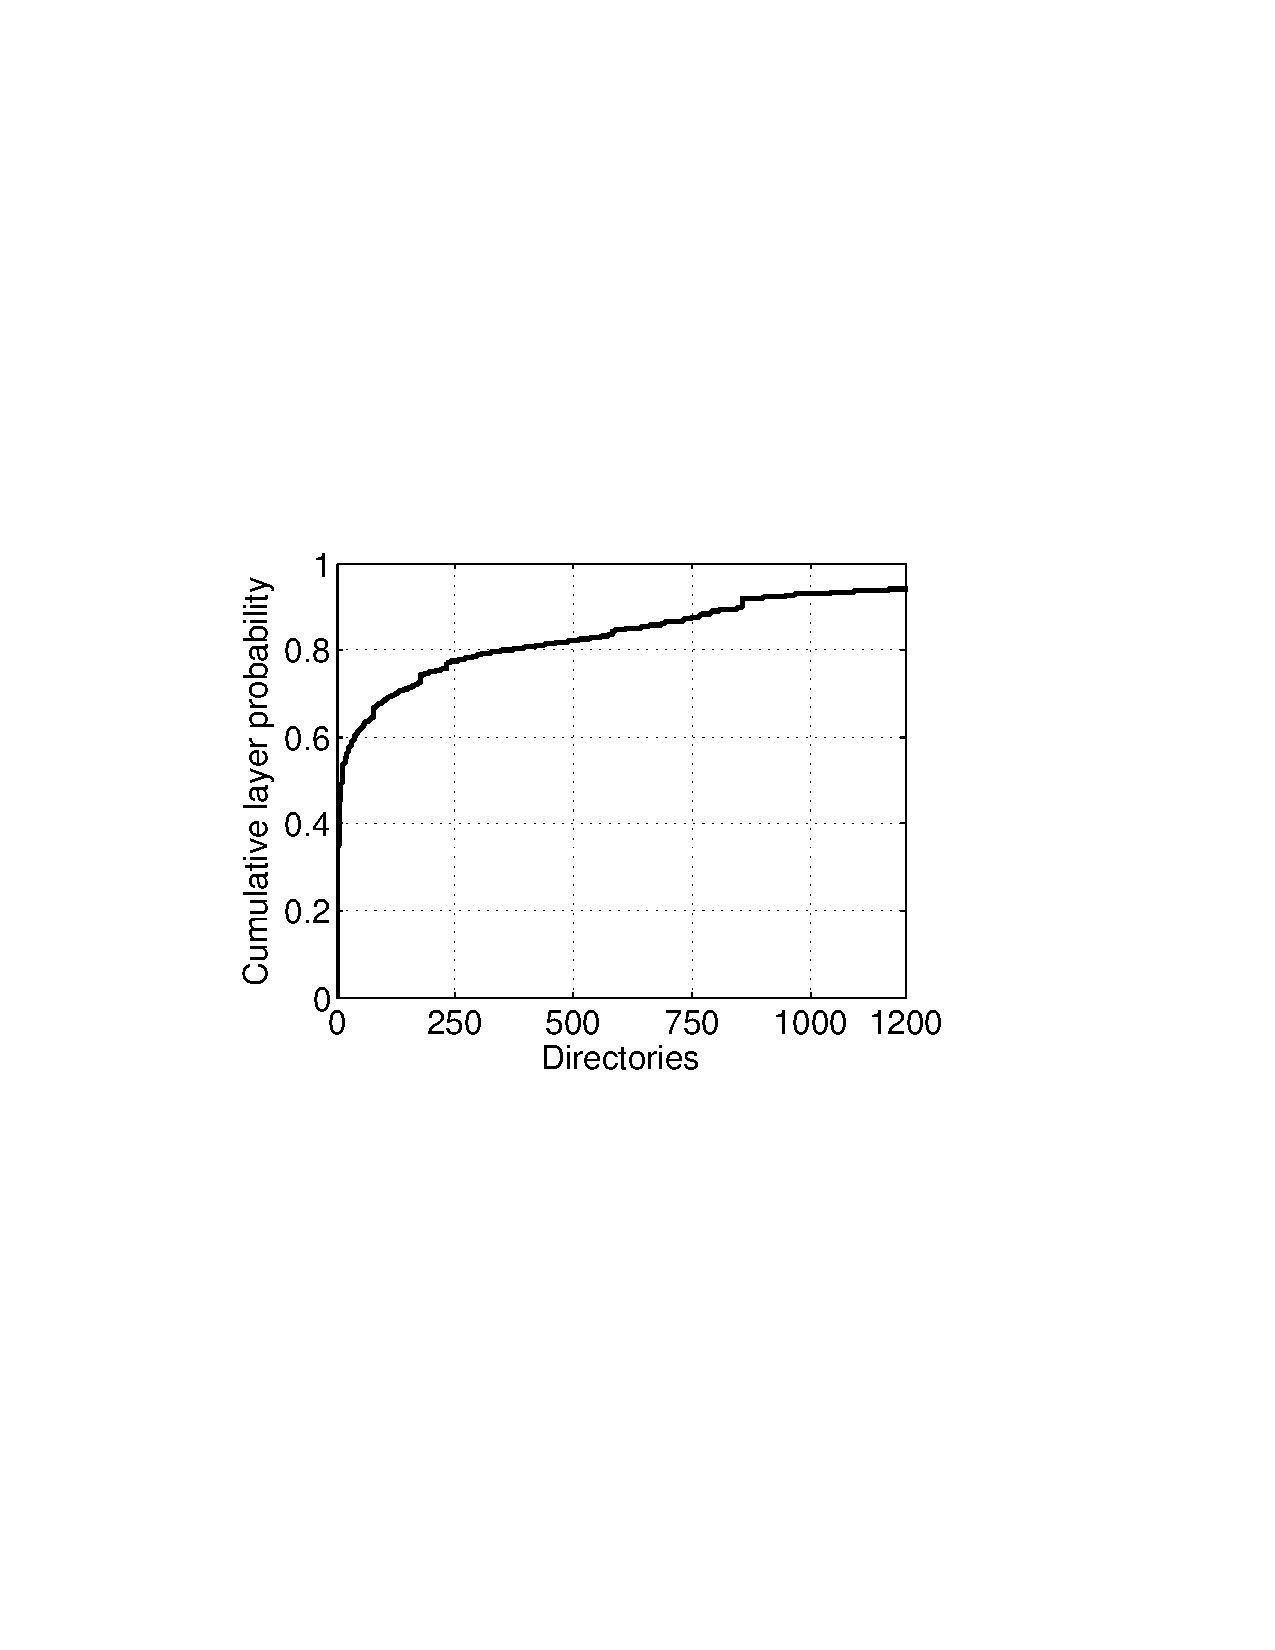
\includegraphics[width=1\textwidth]{graphs/dir_cnt.pdf}
		\caption{Directory count distribution}
		\label{fig_dir_cnt}
	\end{minipage}%
	\begin{minipage}{0.26\textwidth}
		\centering
		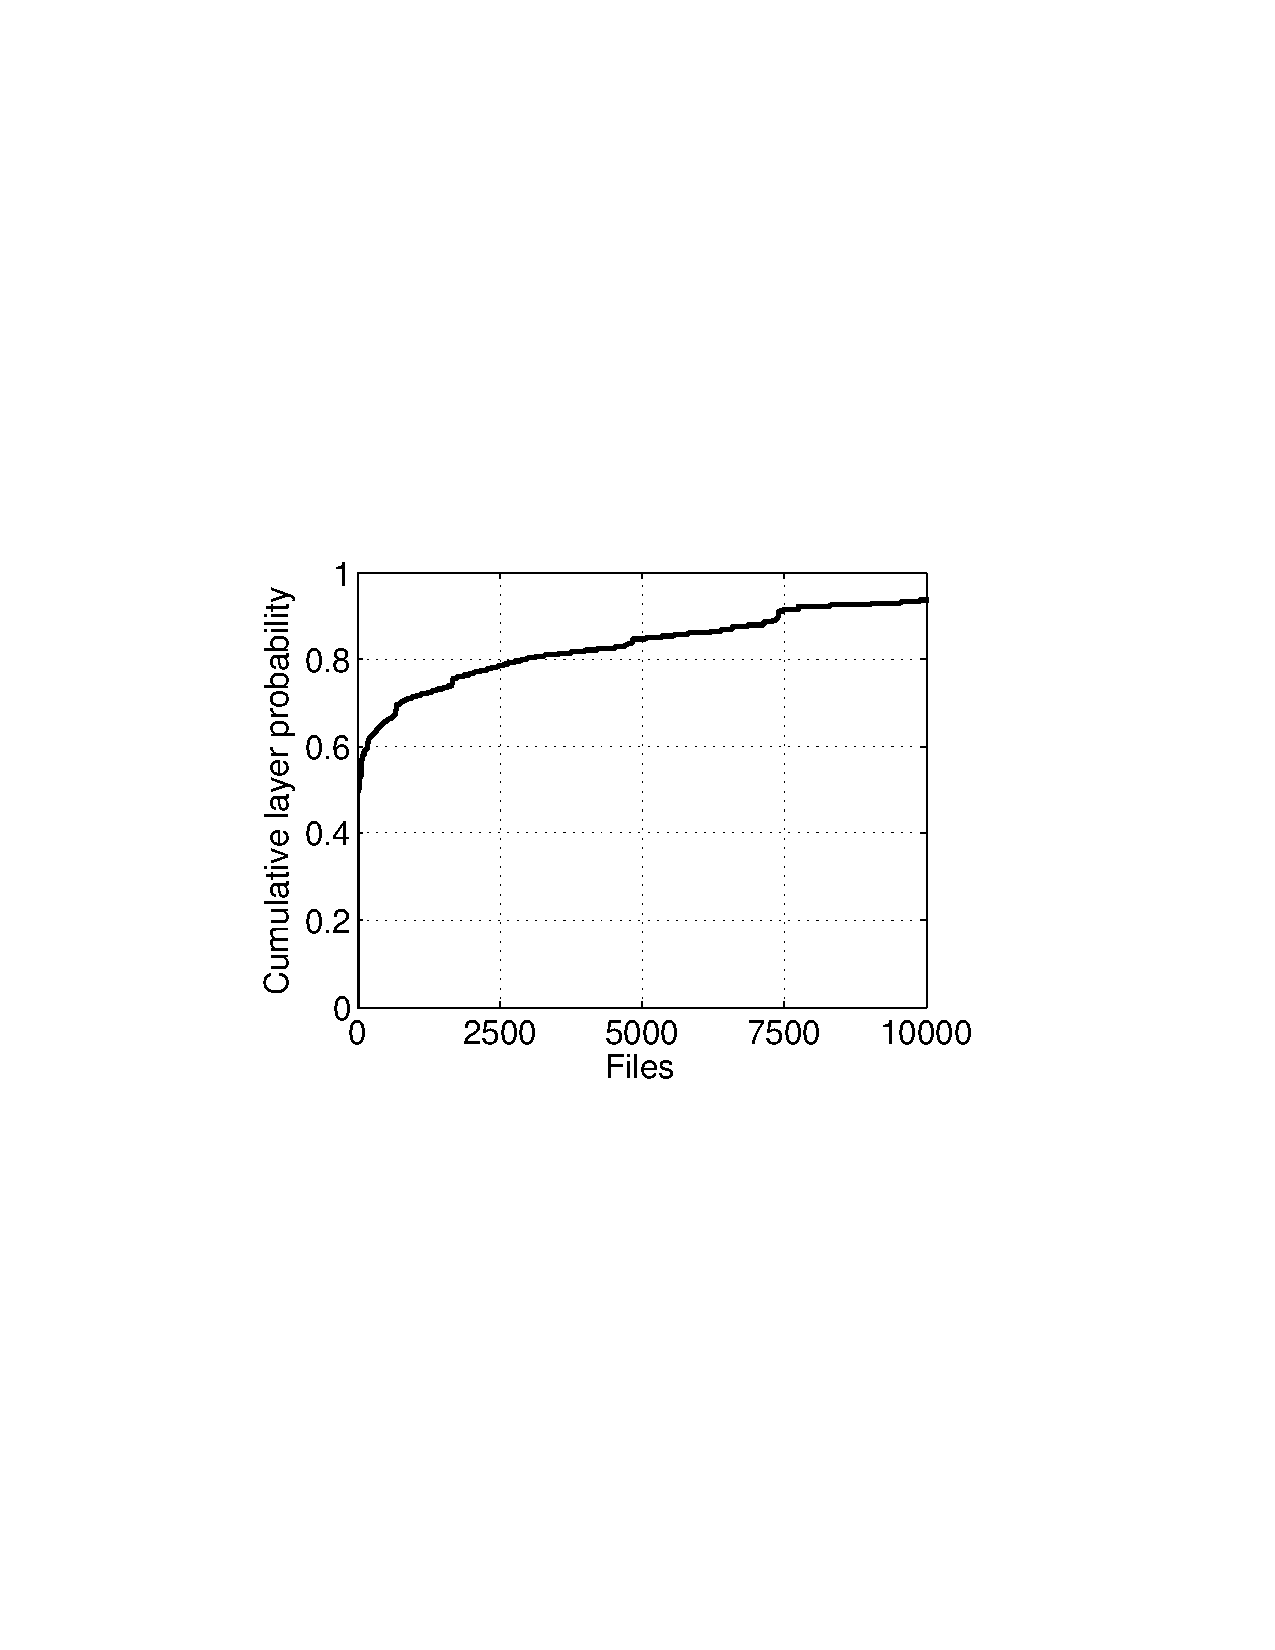
\includegraphics[width=1\textwidth]{graphs/file_cnt.pdf}
		\caption{File count distribution}
		\label{fig_file_cnt}
	\end{minipage}
\end{figure}

\subsubsection{File count distribution}

Figure~\ref{fig_file_cnt} shows the cumulative image frequency by files. 90\% of images have less than 7,410 files. Half of images have less than 30 files. The maximum is 826,196 while the minimum is 1. The average is 2,200.

\subsection{File}

\subsubsection{File size distribution}

\begin{figure}[!t]
	\centering
	\subfigure[CDF of files by file size (KB)]{\label{fig_cdf_file_size_kb}
		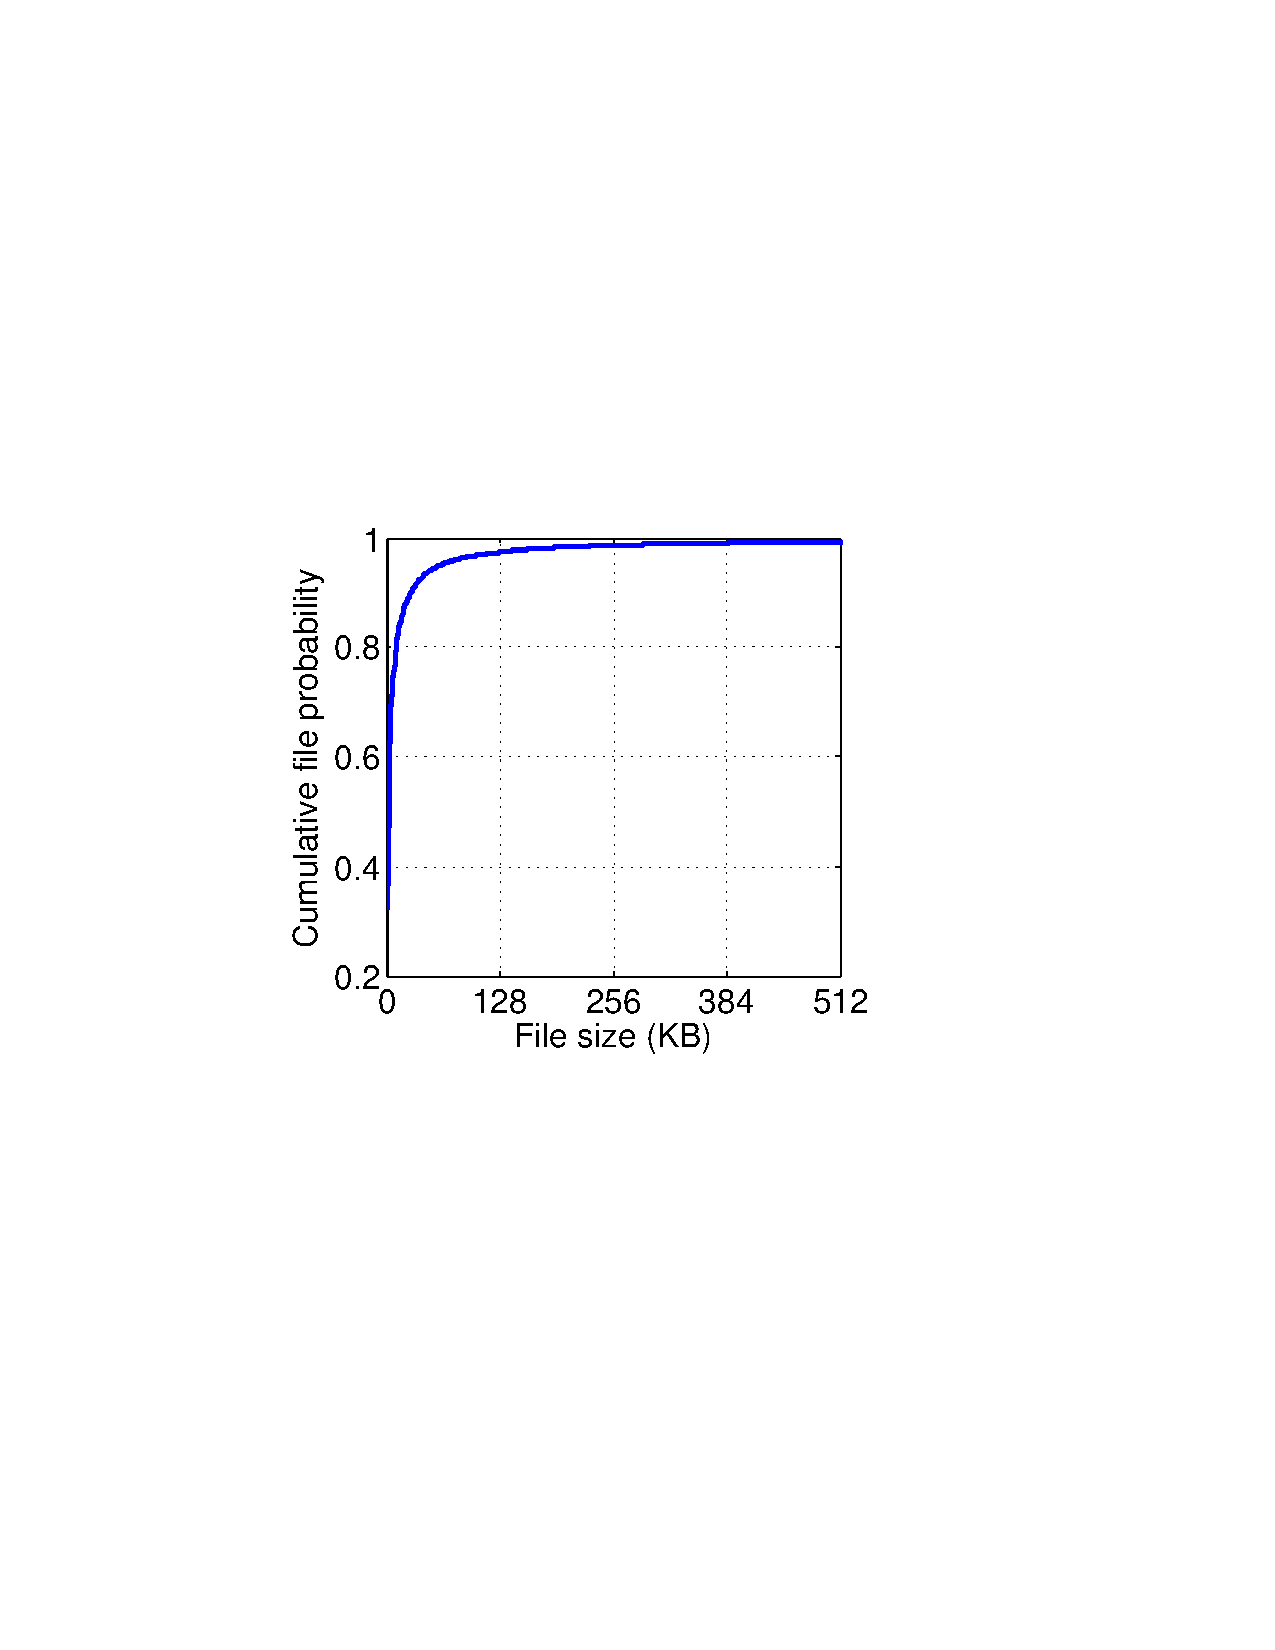
\includegraphics[width=0.23\textwidth]{graphs/cdf_file_size_kb.pdf}
	}
	\subfigure[Histogram of files by file size (KB)]{\label{fig_hist_file_size_kb}
		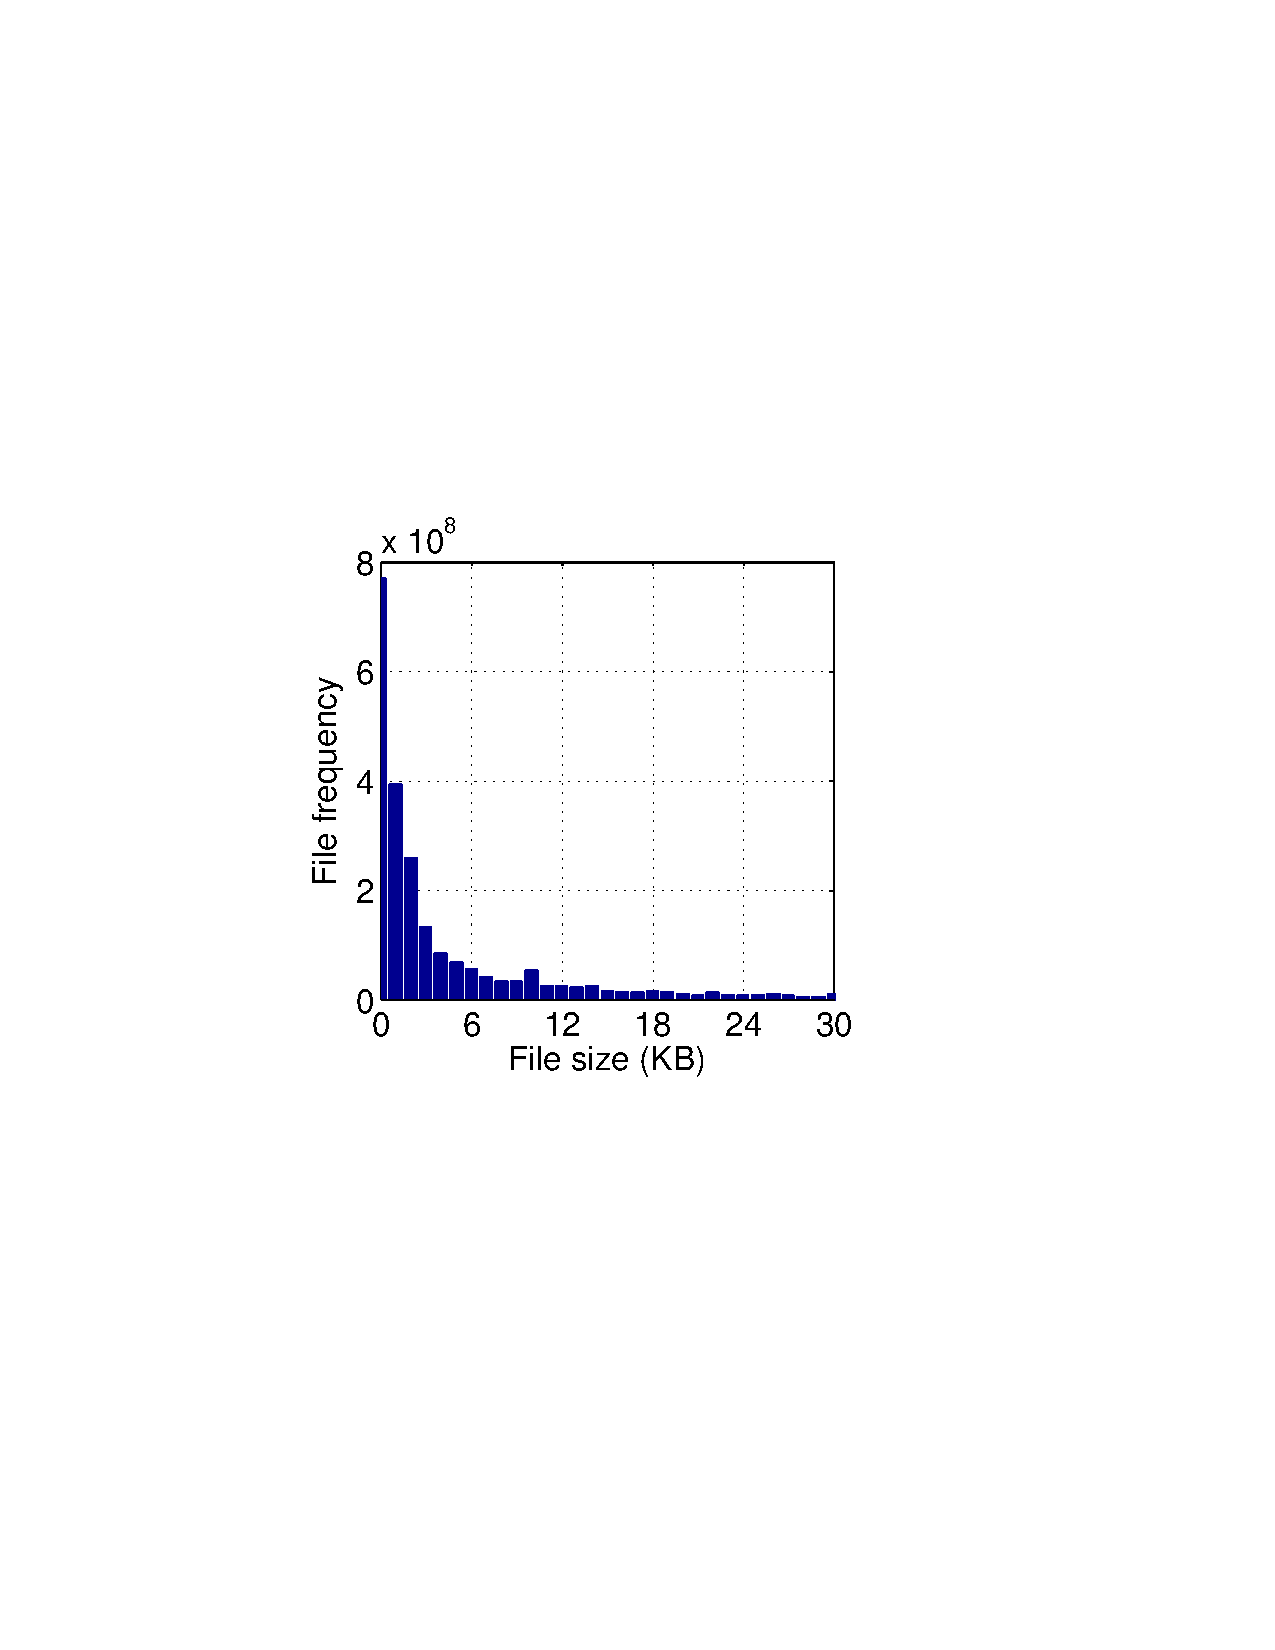
\includegraphics[width=0.22\textwidth]{graphs/hist_file_size_kb.pdf}
	}
	\caption{File size distribution}
	\label{fig-file-size}
\end{figure}

Figure~\ref{fig_cdf_file_size_kb} shows the cumulative file probability by file size. Around 90\% of layers' directory depth is less than 30 KB. 50\% of layers' directory depth is less than ~3. Figure~\ref{fig_hist_file_size_kb} shows the histogram of files by file size. About 769,000,000 files' size is less 1 KB, which is the peak value in the figure. The maximum file size is ~12GB.

Figure~\ref{fig-file-size} suggests that majority of files in Docker images are small files. About 30\% of files are less than 1 KB. 99\% of files are smaller than 1 MB.

\subsubsection{File type distribution}

We use python library named python-magic~\cite{xxx} to obtain the file type. Overall, there are 3,006,619,271 regular files and 282,379,663 symbolic links. Figure~\ref{fig-file-type} shows the top 22 file types. As shown, ASCII text is the most popular file type in Docker images. Around 886,843,570 (30\%) of files are ASCII text files. 
About 322,404,420 (11\%) files are gzip compressed files 
Interestingly, about 22,492,597 (1\%) of files are empty.  

\begin{figure*}
	\centering
	% Requires \usepackage{graphicx}
	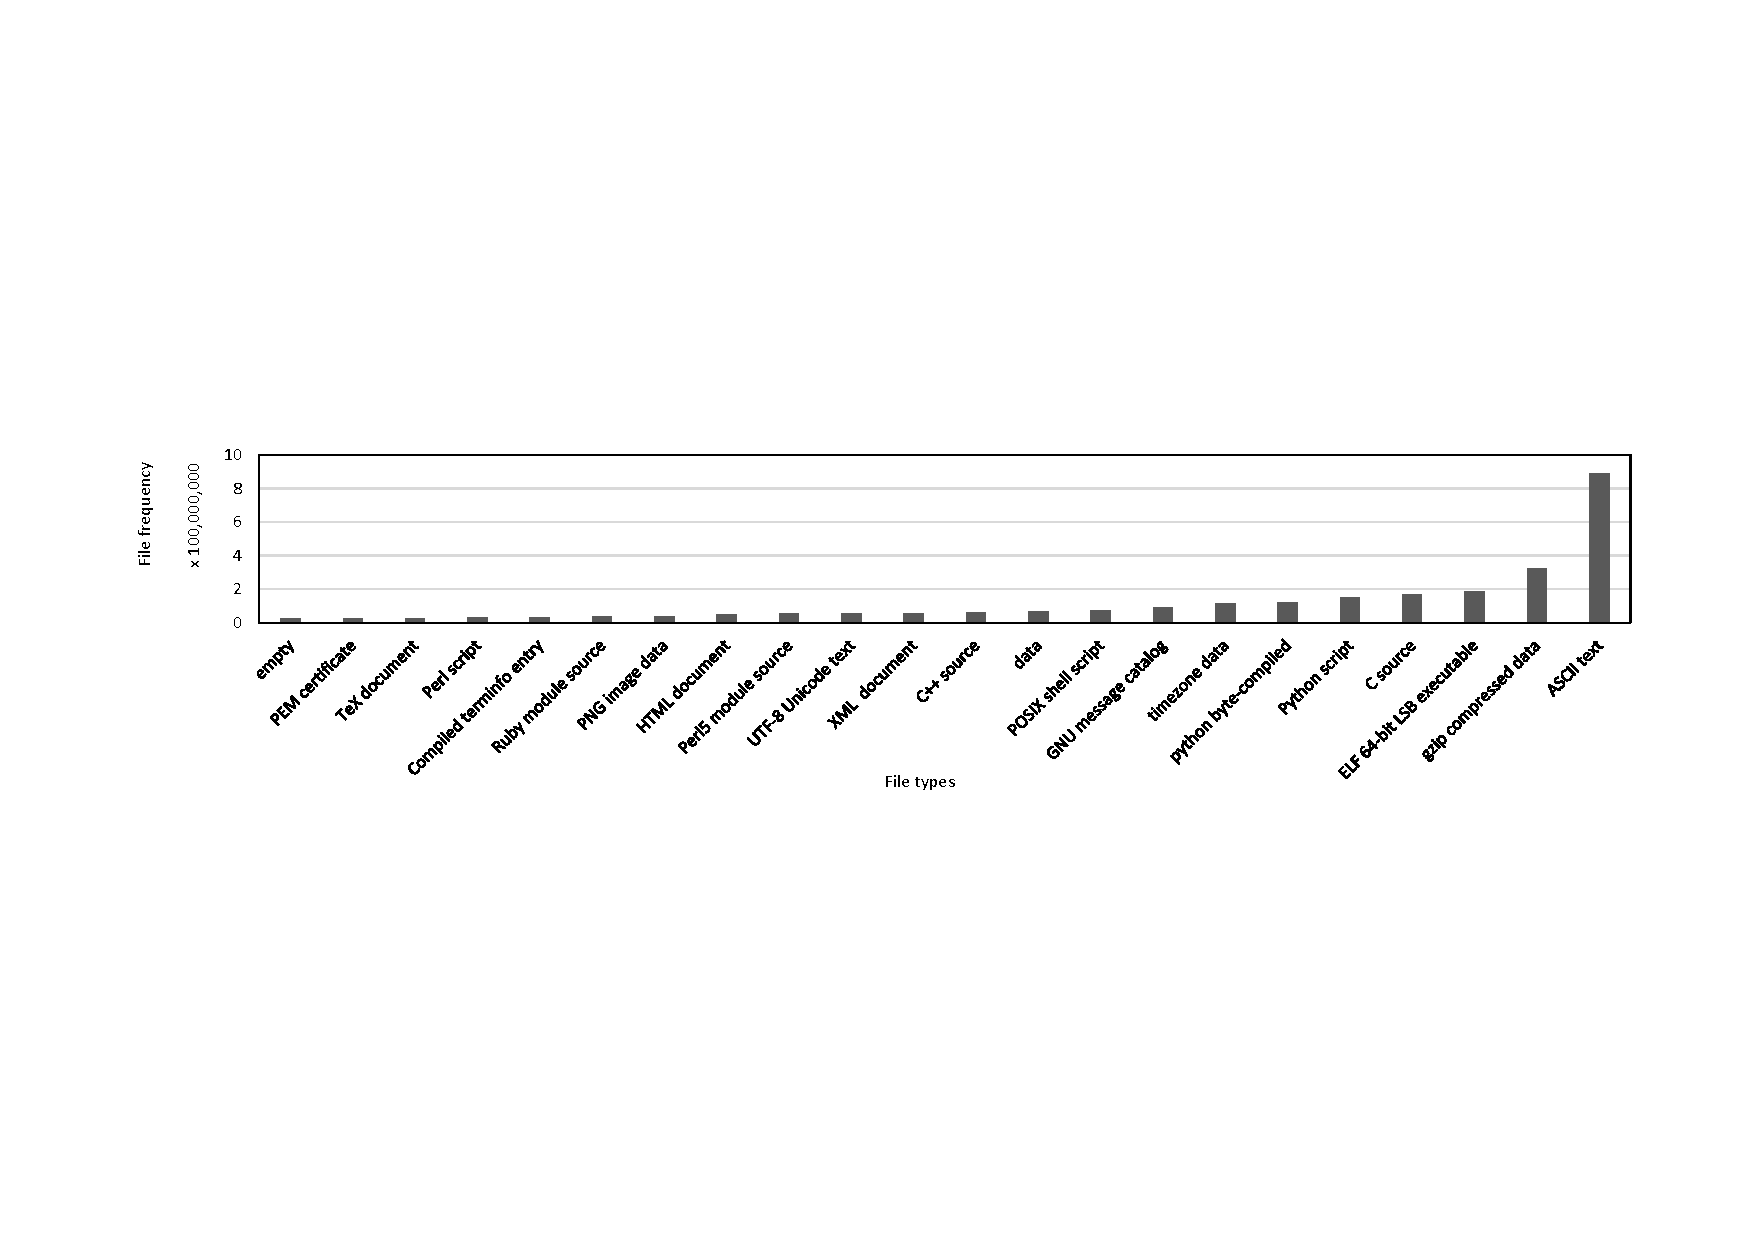
\includegraphics[width=1\textwidth]{graphs/file_type.pdf}\\
	\caption{File type distribution}\label{fig-file-type}
\end{figure*}

%\subsubsection{Repeat file count distribution}
